
\tableofcontents

Schemes were first introduced in their current generality by Grothendieck with
the goal of uniting number theory with geometry. In this article, we will first
discuss what we are looking for in a "geometric object", with subsets of
Euclidean space as motivation, leading us to the definition of a locally ringed
space. At this point, we will have enough to state 
the "Spec, global adjunction", 
which roughly says that there is a functor turning rings into
spaces, Spec, that is "inverse" to taking the ring of global functions on a
space.

The spaces yielded by Spec are what are called affine schemes, and
spaces that are locally affine schemes, are the schemes. 
This is analogous to how manifolds are defined to be spaces that are locally
Euclidean. Along the way, I will showcase some basic but important ideas such as
infinitesimals, which under the language of schemes generalise to seemingly
non-geometric situations. The approach taken is light on sheaf theory, so it
won't be like choking on Hartshorne.

Briefly, here are some of the terminology and notation I will be using : 
\begin{itemize}
  \item For a category $\CC$, $X \in \CC$ means $X$ is an object of $\CC$.
  \item Given a category $\CC$, $\CC$-morphisms refer to morphisms in $\CC$.
  \item Given a category $\CC$ and $X, Y \in \CC$, 
  $\CC(X,Y)$ means the set of $\CC$-morphisms from $X$ to $Y$.
  \item For $X \in \CC$ in a category,
  $\id{X}$ denotes the identity morphism of $X$.
  \item Given a topological space $X$, $\tau_X$ denotes its topology,
  i.e. the set of its opens.
  \item ``Rings'' will always refer to commutative rings with unity. 
  \item $\SET, \TOP, \RING$ denotes respectivly the category of 
  sets, topological spaces, and rings.
  \item ``UP'' is short for universal property. 
\end{itemize}

\section{Locally Ringed Spaces}

To talk about geometry, 
we need to decide on what a ``geometric object'' is to be.
Let us consider the following example and extract some desired properties.

\begin{eg}
  
  Let $X \subs \R^n$.
  \begin{itemize}
    \item (Topology) We have $\tau_X$, the topology of $X$, 
    consisting of opens of $X$. 

    \item (Sheaf of Rings) Given $U \in \tau_X$,
    let $\OO_X(U) := \TOP(U,\R)$ the set of continuous maps $U \to \R$.
    Since $\R$ is a field, 
    $\OO_X(U)$ forms a ring under pointwise addition and multiplication.
    We refer to $f \in \OO_X(U)$ as \emph{functions on $U$}.
    In particular, $f \in \OO_X(X)$ are called \emph{global functions}.

    Given an inclusion of opens $V \subs U$,
    restricting $f \in \OO_X(U)$ to $V$ gives 
    a map $\OO_X(U) \to \OO_X(V)$, which is immediately a ring morphism
    and in particular the identity when $U = V$.
    What's more, the restriction ring morphisms are compatible with 
    ``triangles of inclusions'' : 
    \begin{cd}
      U                 &           & & \OO_X(U) \ar[dd] \ar[dr] & \\
                        & V \ar[ul] & \rightsquigarrow & & \OO_X(V) \ar[dl] \\
      W \ar[uu] \ar[ur] &           & & \OO_X(W) &
    \end{cd}
    I will use $\fall{V}{U} f$ to denote the restriction of 
    a function $f$ on $U$ to a smaller open $V$.
    
    Furthermore, 
    given any open $U$, an open cover $\UU$ of $U$,
    and a collection of functions $(f_V) \in \prod_{V \in \UU} \OO_X(V)$
    that agree on intersections,
    you can ``glue'' $(f_V)$ uniquely to 
    a function $f \in \OO_X(U)$,
    which is to say there exists a unique $f \in \OO_X(U)$ such that
    for all $V \in \UU$, $\fall{V}{U} f = f_V$.

    The collection of the above data,
    information $\OO_X(U)$ on opens that behave like functions in the sense of 
    restrictions and unique gluing,
    is what we call a \emph{sheaf of rings on $X$}.

    \item (Residue Fields, Evaluation, Jointly Surjective)
    
    Let $x \in X$ be a point.
    Then given any open neighbourhood $U$ of $x$,
    we have evaluation at $x$, $(\ev_x)_U : \OO_X(U) \to \R, f \mapsto f(x)$,
    which is in fact a ring morphism. 
    
    Furthermore, for any inclusion of open neighbourhoods $V \subs U$ of $x$,
    restriction commutes with evaluation at $x$ : 
    \begin{cd}
      \OO_X(U) \ar[rd,"(\ev_x)_U"] \ar[dd] & \\
      & \ka(x) \\
      \OO_X(V) \ar[ru,"(\ev_x)_V"{swap}]
    \end{cd}
    where we have denoted $\ka(x) := \R$ to emphasize 
    ``these are the numbers you get from evaluating at the point $x$''
    and refer to $\ka(x)$ as the \emph{residue field at $x$}.

    By severe abuse of notation, we write the above 
    as \[
      \ev_x : \OO_X \to \ka(x)
    \]
    Also note that for all $\la \in \ka(x)$,
    there exists a functions $f$ on some open neighbourhood $U$ of $x$
    such that $\ev_x(f) = \la$,
    just because constant functions are also continuous. 
    I refer to this as
    $\ev_x$ being \emph{jointly surjective}.

    \item (Invertible on Open Support)
    Let $f \in \OO_X(U)$ be a function on an open $U$. 
    Define \[
      D(f) := \set{x \in U \st \ev_x(f) \neq 0}
    \]
    i.e. the \emph{support of $f$}.
    By continuity, $D(f)$ is open.
    $f$ is also invertible on $D(f)$.

  \end{itemize}

  Of course, objects without morphisms are no good so 
  let us dicuss morphisms.
  Let $X \subs \R^n$, $Y \subs \R^m$ and 
  let $\OO_X, \OO_Y$ denote 
  their respective structure sheaves of continuous functions.
  Let $\ph : X \to Y$ be a set morphism. 
  \begin{itemize}
    \item (Topological) Since $X$ and $Y$ are topological spaces,
    we will want $\ph$ to be topological as well (which is to say, continuous).
    Since $\ph$ will consist of more data,
    we will use $\ph^\tau$ to denote the topological morphism underlying $\ph$.

    \item (Pullback of Functions)
    Since $\ph \in \TOP(X,Y)$,
    for any open $U$ of $Y$, $\ph$ restricts to 
    a topological morphism $\ph\inv U \to U$ of open sets in $X, Y$.
    In particular, functions on $U$ \emph{pull back} to 
    functions on $\ph\inv U$, i.e. 
    we have a map \[
      \ph^\flat_U : \OO_Y(U) \to \OO_X(\ph\inv U), f \mapsto f \circ \ph
    \]
    which is in fact a ring morphism.
    Furthermore, this commutes with restriction : 
    \begin{cd}
      \OO_X(\ph\inv U) \ar[d] & \ar[l,"\ph^\flat_U"{swap}] \ar[d] \OO_Y(U) \\
      \OO_X(\ph\inv V) & \ar[l,"\ph^\flat_V"] \OO_Y(V)
    \end{cd}

    Combining the technique of abuse of notation and writing backwards,
    we write the above as : \[
      \OO_X \circ \ph\inv \leftarrow \OO_Y : \ph\flat
    \]
    We will call $\ph^\flat$ the 
    \emph{pullback on functions along $\ph$}.

    \item (Commuting with Evaluation and Pullback of Residue Fields)
    Let $x$ be a point of $X$.
    Then any function $f$ around $\ph(x)$ pulls back to a function 
    around $x$. 
    Furthermore, $\ev_x(f \circ \ph\inv) = \ev_{\ph(x)}(f)$. 
    That is to say, we have the following commutative square 
    (using abuse of notation) : 
    \begin{cd}
      \OO_X\circ\ph\inv \ar[d,"\ev_x"{swap}] & 
      \OO_Y \ar[l,"\ph^\flat"{swap}] \ar[d,"\ev_{\ph(x)}"] \\
      \ka(x) & \ar[l,"\ph^\ka_x"] \ka(\ph(x))
    \end{cd}
    where $\ka(x) = \ka(\ph(x))$ and $\ph^\ka_x = \id{\R}$.
    We will call the collection of data $\ph^\ka = (\ph^\ka_x)_{x \in X}$ the 
    \emph{pullback of residue fields}. 
    
  \end{itemize}

\end{eg}

Abstracting these properties gives us 
the definition of the \emph{category of locally ringed spaces}.

\begin{dfn}[Category of Locally Ringed Spaces]
  
  A \emph{locally ringed space}\footnote{
    This is not the standard definition of locally ringed spaces,
    though it is equivalent. 
    The standard definition packs
    the data of residue fields, jointly surjective evaluations,
    and functions invertible on their open supports into 
    a single condition of ``stalks of $\OO_X$ being local rings''.
    This is more economic, however,
    it requires building new intuition about stalks and local rings.
    The advantage of the definition presented here is that 
    most people already have intuition about evaluating functions at points. 
  } consists of the following data : 
  \begin{itemize}
    \item (Underlying Topological Space) $X \in \TOP$. 
    \item (Structure Sheaf) 
    On every open $U$ of $X$, we have a ring $\OO_X(U)$,
    the \emph{ring of functions on $U$} and 
    we have \emph{restriction ring morphisms} from 
    larger opens to smaller opens that commute. 
    In abstract non-sense, $\OO_X$ is a functor from 
    the dual category of $\tau_X$ to $\RING$ : 
    \[\OO_X : \tau_X\op \to \RING\]
    We require $\OO_X$ to have the \emph{sheaf property},
    that is, functions unique glue on any open cover of any open.
    It is convention to have $\OO_X(\nothing) = 0$.
    \item (Residue Fields) for every $x \in X$, a field $\ka(x)$.
    This is the \emph{residue field at $x$}.
    \item (Jointly Surjective Evaluation) For every point $x \in X$, 
    a collection of evaluation ring morphisms on open neighbourhoods of $x$
    that is jointly surjective onto $\ka(x)$ : 
    \[
      \ev_x : \OO_X \to \ka(x)
    \]
    \item (Invertible on Open Support)
    For every $f \in \OO_X(U)$ on some open $U$,
    its support \[
      D(f) := \set{x \in U \st \ev_x(f) \neq 0}
    \]
    is open and $f$ is invertible on $D(f)$.
  \end{itemize}
  For the structure sheaf, it is convention for $\OO(\nothing) := 0$.
  Open sets of the form $D(f)$ are called \emph{basic opens}.

  A morphism of locally ringed spaces $\ph : X \to Y$ consists of 
  the following data : 
  \begin{itemize}
    \item (Underlying Topological Morphism) $\ph^\tau \in \TOP(X,Y)$
    \item (Pullback of Functions) 
    a collection of ring morphisms from $\OO_Y$ to $\OO_X \circ {\ph^\tau}\inv$
    that commute with restriction : 
    \[
      \OO_X \circ \ph\inv \leftarrow \OO_Y : \ph\flat
    \]
    \item (Pullback of Residue Fields and Evaluation)
    For every point $x \in X$,
    we require a ring morphism $\ph^\ka_x$ that commutes with 
    evaluation at $x$ and $\ph(x)$ : 
    \begin{cd}
      \OO_X\circ\ph\inv \ar[d,"\ev_x"{swap}] & 
      \OO_Y \ar[l,"\ph^\flat"{swap}] \ar[d,"\ev_{\ph(x)}"] \\
      \ka(x) & \ar[l,"\ph^\ka_x"] \ka(\ph(x))
    \end{cd}
  \end{itemize}
  The above defines the \emph{category of locally ringed spaces},
  denote $\LRSP$.
\end{dfn}

\begin{rmk}
  Locally ringed spaces are what we think of as ``geometric objects''.
  In particular, 
  topological manifolds, smooth manifolds, complex manifolds 
  are all examples of locally ringed spaces. 
  In fact, you can define them \textit{using} locally ringed spaces.  

  For this, we need the following. 
  Given $X \in \LRSP$, $U \in \tau_X$,
  $\tau_U \subs \tau_X$. 
  Then restricting the structure sheaf of $X$ to the opens of $U$ and 
  using the residue fields as you already have,
  $(U,\res{\OO_X}{\tau_U},(\ka(x))_{x\in U})$ is 
  naturally a locally ringed space.

  With the above, we have the equivalence of the following data : 
  \begin{align*}
    &M \in \MFD, C^\infty\MFD, \C\MFD \iff \\
    &M \in \LRSP \text{ and }
    \forall\, x \in M, \exists\, U_x \in \tau_M ,
    x \in U_x \text{ and }
    U_x \iso_\LRSP  (\R^n, C^0), (\R^n, C^\infty), (\C^n, \OO_{hol}) \\
    & (\text{+ Haudorff, Paracompact})
  \end{align*}
  Here $(\R^n,C^0), (\R^n, C^\infty), (\C^n, \OO_{hol})$ are
  $\R^n$ and $\C^n$ with the sheaves of 
  continuous $\R$-valued functions, smooth functions, holomorphic functions.

  I think of this as
  choosing different ``local models'' for our geometric objects,
  each giving rise to a different geometry. 
  \[
  \begin{matrix}
    \text{``Geometry''} &
    \textit{Why} & 
    \text{Diff. Geom.} & 
    \text{Complex Geom.} & 
    \text{Alg. Geom.} \\
    \text{``Local Model''} &
    (\R^n, C^0) & 
    (\R^n, C^\infty) & 
    (\C^n, \OO_{hol}) & 
    \textit{???}
  \end{matrix}
  \]
  At this point, 
  we're actually one step away from giving the definition of a scheme;
  we just need the ``local model'' that gives algebraic geometry.
  These are the \emph{affine schemes}.

\end{rmk}
\begin{rmk}[On Atlases]
  For the differential geometers, 
  an smooth atlas allows you to define a structure sheaf consisting of 
  ``functions smooth with respect to the atlas''.
  Then two atlases are equivalent if and only if 
  they give rise to isomorphic structure sheaves,
  i.e. the same ``smooth structure''.
  In particular, 
  each equivalence class of atlases turns out to have 
  a unique maximal element.
  I like to think of this as why maximal atlases are called 
  smooth structures.

  The above works for holomorphic charts as well, 
  giving rise the structure sheaf of holomorphic functions. 
\end{rmk}

\section{Affine Schemes and the $\spec$, Global Function Adjunction}

\begin{rmk}
  
  Let $X,Y$ be locally ringed spaces. 
  Then given a morphism $\ph : X \to Y$ of locally ringed spaces,
  we have the pullback of global functions 
  $\ph^\flat_Y : \OO_Y(Y) \to \OO_X(X)$.
  \begin{cd}
    \LRSP \ar[r,"\OO_\star(\star)", squiggly] & \RING\op \\
    X \ar[d,"\ph"] & \OO_X(X) \\
    Y & \OO_Y(Y) \ar[u,"\ph^\flat_Y"{swap}]
  \end{cd}
  This gives a functor \[
    \OO_\star(\star) : \LRSP \to \RING\op, 
    X \mapsto \OO_X(X)
  \]
  reversing directions of morphisms.
  I will refer to this as the ``Global Functions Functor''.

  The question that affine schemes address is the following : 
  Suppose we are given a ring morphism $\ph^\bot : A \to \OO_X(X)$.
  \begin{cd}
    \LRSP & \RING\op \ar[l,squiggly] \\
    X \ar[d,"\ph"] & \OO_X(X) \\
    Y & A = \OO_Y(Y) 
      \ar[u,"\ph^\bot = \ph^\flat_Y"{swap}]
  \end{cd}
  Can we make a locally ringed space $Y$ 
  recovering $A = \OO_Y(Y)$ as its ring of global functions,
  such that there exists a unique morphism $\ph : X \to Y$
  recovering our initial ring morphism $\ph^\bot : A \to \OO_X(X)$
  as the pullback of global functions? 
  The answer is \emph{yes}.
  This is precisely the so called... 
\end{rmk}

\begin{prop}[$\spec$, Global Function Adjunction]
  
  There exists a functor $\spec : \RING\op \to \LRSP$ such that
  for any $X \in \LRSP$ and $A \in \RING$, 
  $A = \OO_{\spec A}(\spec A)$ and 
  we have the bijection 
  \begin{align*}
    \LRSP(X,\spec A) &\iso \RING(A,\OO_X(X)) \\
    \ph &\mapsto \ph^\flat_{\spec A}
  \end{align*}

  Locally ringed spaces isomorphic to $\spec A$ for some ring $A$ 
  are called \emph{affine schemes}.
\end{prop}

\begin{rmk}
  The affine schemes are, in some sense, 
  locally ringed spaces whose data consists of nothing more than
  its ring of global functions.
  That is to say, ``their geometry is determined by their algebra''.
  This is why they're the ``local model'' of algebraic geometry. 
  With this, you can probably guess what the definition of a scheme is. 
\end{rmk}

\begin{dfn}[Schemes]
  
  Let $X \in \LRSP$. 
  Then $X$ is called a \emph{scheme} when 
  for all points $x \in X$, 
  there exists an open neighbourhood $U_x$ of $x$ that is 
  an affine scheme with its obvious locally ringed space structure. 
\end{dfn}

\begin{rmk}
  
  So schemes are not so different from manifolds.
  They are both locally ringed spaces,
  just ``locally modeled'' differently. 
  It is also in this sense that ``commutative algebra is 
  the calculus of schemes''.
  Calculus is the geometry of $(\R^n,C^\infty)$ and 
  commutative algebra is the geometry of affine schemes. 

  The construction of the functor $\spec$ will occupy the remainder 
  of the document. 
  We proceed in steps.
  First, we will make the functor $\spec : \RING\op \to \SET$,
  then $\spec : \RING\op \to \TOP$,
  and finally, $\spec : \RING\op \to \LRSP$ and prove the adjunction. 
  Along the way, 
  I hope to show you geometric interpretations of 
  some algebraic notions. 
  \begin{cd}
    \spec : \RING\op \ar[r] \ar[rd] \ar[rdd] & \SET \\
    & \TOP \ar[u] \\
    & \LRSP \ar[u]
  \end{cd}

\end{rmk}

\section{Set-theoretic $\spec$}

\begin{rmk}
  The data of a set consists of nothing more than its elements.
  So the question is : 
  given $A \in \RING$, what are the points of $\spec A$?

  We proceed by wishful thinking and assume we have $\spec A$ already, 
  satisfying the adjunction. 
  Take $p \in \spec A$.
  You think hard about what you can do with a point in a locally ringed space.
  Then you realize, the only thing you can do is evaluate functions 
  around $p$. 
  \[
    \ev_p : \OO_{\spec A} \to \ka(p)
  \]
  After staring at this for a long time, 
  you'll then realize that because this is happening in $\RING$,
  you are looking at things backwards; 
  you should reading the evaluation like : 
  \[
  \ka(p) \leftarrow \OO_{\spec A}: \ev_p
  \]
  It may then dawn on you that 
  this looks like the pullback of functions along 
  a morphism from some space into $\spec A$.
  What space? 
  Well,
  it needs to have its structure sheaf be 
  given by only $\ka(p)$ on all (non-empty) opens. 
  So what better space to take than the singleton.
  \[ p : \bullet_{\ka(p)} \to \spec A \]
  In more detail, 
  the single space $\bullet_{\ka(p)}$ has 
  structure sheaf given by $\OO_{\bullet_{\ka(p)}}(\bullet) := \ka(p)$
  and residue field $\ka(\bullet) := \ka(p)$.
  In particular, 
  we see that under the adjunction, 
  the morphism of ringed spaces $p : \bullet_{\ka(p)} \to \spec A$
  corresponds to $\ev_p : A \to \ka(p)$,
  a ring morpshism from $A$ into a field. 
  \begin{cd}
    \LRSP & \RING\op \\
    \bullet_{\ka(p)} \ar[d,"p"] & \ka(p) \\
    \spec A & A \ar[u,"\ev_p"{swap}]
  \end{cd}

  Conversely, 
  given a ring morphism $\ev : A \to K$ into a field $K$,
  we can consider the singleton space $\bullet_K$
  with structure sheaf and residue field $K$.
  Then the adjunction gives a morphism of locally ringed spaces 
  $\io_K : \bullet_K \to \spec A$,
  giving us a point $\io_K(\bullet)$.
  So we have a surjection : 
  \[
    \set{A \to K \st K \text{ field}} \twoheadrightarrow \spec A,
    \brkt{\ev_K : A \to K} \mapsto \io_K(\bullet)
  \]
  Surjections are precisely equivalence relations,
  in other words, 
  this suggests $\spec A$ should be 
  maps from $A$ into fields up to some equivalence. 
  It is the following.

  Given $\ev_K : A \to K$ where $K$ is a field.
  If $\io_K(\bullet) = p$ then 
  part of the data of $\io_K$ \textit{includes a pullback of residue fields 
  $(\io_K)^\ka_\bullet : \ka(p) \to K$}.
  This gives the data of the commuting triangle on the left : 
  \begin{cd}
    & \LRSP & \RING\op & \\
    \bullet_{K} \ar[dr,"\io_K"{swap}] \ar[r] 
    & \bullet_{\ka(p)} \ar[d,"p"] 
    & \ka(p) \ar[r,"\io^\ka_\bullet"] & K \\
    & \spec A & A \ar[ru,"\ev_K"{swap}] \ar[u,"\ev_p"] & 
  \end{cd}
  and this corresponds to the triangle on the right by the adjunction. 
  So \[
    \io_K(\bullet) = p \implies \ev_K \text{ factors through } \ev_p
  \]
  Conversely, 
  if we have $\ev_K$ factoring through $\ev_p$ (i.e. the right triangle),
  a morphism $\ka(p) \to K$ again 
  clearly defines a morphism $\bullet_K \to \bullet_{\ka(p)}$.
  Then the left triangle above commutes because 
  through the adjunction,
  both $\io_K$ and the composition $\bullet_K \to \bullet_{\ka(p)} \to \spec A$
  correspond to $\ev_K$, and hence must be equal by the adjunction. 
  Thus we have 
  \[
  \io_K(\bullet) = p \iff \ev_K \text{ factors through } \ev_p
  \]
  which is to say, 
  ``$\ev_p$ is the minimal representative in its equivalence class''.
  It is not hard to see that 
  this equivalence relation is the same as the one generated by 
  $(A \to K) \sim (A \to L) := \exists\, K \to L, $
  \begin{cd}
    K \ar[r] & L \\
    A \ar[u] \ar[ur] & 
  \end{cd}
  where $K, L$ are fields. 
  We have our definition. 
  % So we guess that : 
  % \[
  %   \spec A \map{\sim}{} \set{A \to K \st K \text{ field}},
  %   p \mapsto \ev_p
  % \]
  % However, if we have two ring morphisms into fields 
  % with a ring morphism in between : 
  % \begin{cd}
  %   K \ar[d] & A \ar[l,"\ev_K"{swap}] \ar[ld,"\ev_L"] & 
  %     \rightsquigarrow & \bullet_K \ar[r,"\io_K"] & \spec A\\
  %   L & & & \bullet_L \ar[u] \ar[ur,"\io_L"{swap}] & 
  % \end{cd}
  % then the adjunction gives the commutative triangle on the right,
  % implying $\io_L(\bullet) = \io_K(\bullet)$.
  % This suggests we should quotient 
  % the set of ring morphisms from $A$ into fields by
  % the equivalence relation generated by 
  % $(\ev_K : A \to K) \sim (\ev_L : A \to L)$ when 
  % there exist $K \to L$ such that 
  % \begin{cd}
  %   K \ar[d,"\ph"{swap}] & A \ar[l,"\ev_K"{swap}] \ar[ld,"\ev_L"] \\
  %   L & 
  % \end{cd}
  % This will actually look like 
  % having a ``zig-zag'' of fields in between : 
  % \begin{cd}
  %   K & & &             & \bullet_K \ar[rd] \ar[rrdd, bend left = 45] & & \\
  %   & K_1 \ar[lu] \ar[ld] & & & & \bullet_{K_1} \ar[rd] & \\ 
  %   \vdots & & A \ar[lluu, bend right = 45] \ar[lldd,bend left = 45]
  %     \ar[lu] \ar[ld] \ar[ll]
  %     & \rightsquigarrow & \vdots \ar[ru] \ar[rd] \ar[rr] & & 
  %     \spec A \\
  %   & K_n \ar[lu] \ar[ld] & & & & \bullet_{K_n} \ar[ru] &   \\
  %   L & & & & \bullet_L \ar[ru] \ar[rruu,bend right = 45] & &     
  % \end{cd} 
  % which under the adjunction turns into 
  % a ``zig-zag'' of inclusion of points. 
  % It then follows that 
  % \[
  %   \spec A \map{}{} \set{A \to K \st K \text{ field}} / \sim,
  %   p \mapsto [\ev_p]
  % \]
  % is an injection. 
  % It is also a surjection : 
  % given a ring morphism $\ev_K : A \to K$ into a field, 
  % the data of the adjunct $\io_K : \bullet_K \to \spec A$ 
  % includes commutativity of evaluation with the pullback of residue fields : 
  % \begin{cd}
  %   \OO_{\bullet_K}\circ\io_K\inv \ar[d,"\ev_{\bullet}"{swap}] & 
  %   \OO_{\spec A} \ar[l,"\io_K^\flat"{swap}] \ar[d,"\ev_{\io_K(\bullet)}"] \\
  %   \ka(\bullet) & \ar[l,"{\io_K}^\ka_\bullet"] \ka(\io_K(\bullet))
  % \end{cd}
  % which on the global level gives : 
  % \begin{cd}
  %   K \ar[d,"\id{K}"{swap}] & 
  %   A \ar[l,"\ev_K"{swap}] \ar[d,"\ev_{\io_K(\bullet)}"] \\
  %   K & \ar[l,"{\io_K^\ka}_\bullet"] \ka(\io_K(\bullet))
  % \end{cd}
  % Hence, $\io_K(\bullet)$ gives the equivalence class 
  % that $\ev_K : A \to K$ is in. 
  % We have arrived at the definition of the set $\spec A$.
\end{rmk}

\begin{dfn}[Set-theoretic $\spec$]
  
  For $A \in \RING$, 
  define \[
    \spec A := \set{A \to K \st K \text{ field}} / \sim
  \]
  where the equivalence relation is as in the remark. 
  The construction is clearly functorial,
  giving \[
    \spec : \RING\op \to \SET
  \]
\end{dfn}

\begin{rmk}[Worries]

  For those who have already done some modern algebraic geometry, 
  you may be wondering where the prime ideals are,
  since $\spec A$ is more standardly defined as 
  the set of prime ideals of $A$.
  A perhaps more serious question is whether under our definition,
  $\spec A$ is even a set at all?
  
  Both these questions are answered by the following lemma 
  which realizes our idea that for $p \in \spec A$,
  $\ev_p : A \to \ka(p)$ is the minimal representative of $p$.
  
\end{rmk}

\begin{lem}[Evaluation]
  
  Let $A \in \RING$, $p \in \spec A$ be a point.
  Then there exists $\ev_p : A \to \ka(p)$
  where $\ka(p)$ is a field that is minimal in 
  the equivalence class $p$,
  i.e. every other $A \to K$ representing $p$ 
  factors uniquely through $\ev_p$.
  $\ev_p$ is thus unique up to unique isomorphism in the class $p$.
  In fact, $\ev_p$ is an epimorphism of rings. 
  Its codomain $\ka(p)$ is called the \emph{residue field at $p$}.

  Hence, 
  $\spec A$ bijects with the set of prime ideals of $A$.
  
\end{lem}
\begin{proof}
  For any $\ev_K : A \to K$ representing $p$,
  the ideal $I = \ker\ev_K$ is independent of $K$ by 
  the equivalence relation and ring morphisms from fields being injective. 
  Define $\ev_p : A \to \ka(p)$ with $\ka(p) := \text{Frac }A/I$.
  The the UP of quotients and fields of fractions 
  implies the minimality of $\ev_p$ as a representative of $p$.
  $\ev_p$ is indeed epi and $I = \ker\ev_p$.

  Prime ideals inject into $\spec A$ via 
  $\f(p) \mapsto \text{Frac }A/\f(p)$.
  Now for $p \in \spec A$,
  we already saw that $\ka(p) = \text{Frac }A/\ker\ev_p$.
  $\ker\ev_p$ is thus a prime ideal mapping to $p$, proving surjectivity. 
\end{proof}

\begin{rmk}
  Note that given a ring morphism $\ph^\bot : A \to B$
  with corresponding $\ph : \spec B \to \spec A$
  and a point $p \in \spec B$, 
  by minimality of $\ev_{\ph(p)}$,
  we already have the pullback on residue fields : 
  \begin{cd}
    B \ar[d,"\ev_p"{swap}] & A \ar[l,"\ph^\bot"{swap}] \ar[d,"\ev_{\ph(p)}"]\\
    \ka(p) & \ka(\ph(p)) \ar[l,dashed]
  \end{cd}
  Now that we can evaluate functions at points, 
  we're ready to define topological $\spec$.
\end{rmk}

\section{Topological $\spec$}

\begin{prop}[Topological $\spec$]
  
  Let $A \in \RING$.
  For any $f \in A$, 
  define the \emph{support of $f$} to be \[
    D(f) := \set{p \in \spec A \st \ev_p(f) \neq 0}
  \]
  The subsets of $\spec A$ of the above form are called 
  \emph{basic opens}.
  We will use $D(A)$ to denote the set of basic opens. 

  Then the following are true : 
  \begin{itemize}
    \item (Pretopology)
    For all basic opens $U, V \subs \spec A$,
    there exists a basic open $W \subs \spec A$ such that $W \subs U \cap V$.
    In particular, for $f, g \in A$, $D(f) \cap D(g) = D(fg)$.

    Hence $D(A)$ is a pretopology on $\spec A$.
    The topology it generates is called the \emph{Zariski topology},
    the topology initial with respect to basic opens being open. 

    \item (Morphisms)
    Let $\ph^\bot \in \RING(A,B)$ and 
    $\ph^\tau \in \SET(\spec B, \spec A)$ the corresponding map. 
    For $f \in A$, 
    we have \[
      {\ph^\tau}\inv D(f) = D(\ph^\bot(f))
    \]
    Hence, by giving every spectrum the Zariski topology, 
    we have the functor : 
    \begin{cd}
      \RING\op \ar[r,"\spec"] & \TOP 
    \end{cd}
  \end{itemize}

\end{prop}
\begin{proof}
  \textit{(Morphism)}
  For $f \in A$ and $p \in \spec B$,
  $p \in \ph\inv D(f) \iff \ev_{\ph(p)}(f) \neq 0 
  \iff \ev_p(\ph^\bot(f)) \neq 0
  \iff p \in D(\ph^\bot(f))$.
\end{proof}

\begin{rmk}
  Here are some elementary facts about $\spec$ 
  that already starts bridge the gap betweem algebra and geometry.
\end{rmk}

\begin{prop}[Cool Facts]~

  \begin{itemize}
    \item (Non-Zero / Non-empty)
    Let $A \in \RING$.
    Then $A \neq 0$ if and only if $\spec A \neq \nothing$.
    \item (Epimorphisms / Monomorphisms)
    Let $A \to B$ be an epimorphism of rings.
    Then the corresponding $\spec B \to \spec A$ is a monomorphism of 
    topological spaces. 
    In particular, 
    we have the following two examples : 
    \begin{itemize}
      \item (Localization / Zooming in)
      For $B = S\inv A$ with $S \subs A$ multiplicative,
      \[
        \spec S\inv A \map{\sim}{\TOP} \bigcap_{f \in S} D(f)
      \]
      is a topological isomorphism to the subspace. 
      We henceforth identify these. 

      In particular, for a point $p$ and 
      $A_p := S\inv A$ with $S := A\minus\ker\ev_p$,
      $\spec A_p$ is the intersection of all open neighbourhoods of $p$.
      
      \item (Quotient / Closed Subspace)
      For $B = A / I$ for some ideal $I$ of $A$,
      \[
        \spec A / I \map{\sim}{\TOP} V(I)
      \]
      is a topological isomorphism to the closed subspace 
      $V(I) := \set{p \in \spec A \st I \subs \ker\ev_p}$.
      In fact, all closed subsets of $\spec A$ arise this way. 
    \end{itemize}
    \item (Ideal, Subset Adjunction)
    Let $A \in \RING$.
    For any ideal $I \in \ideal(A)$, 
    define \emph{the vanishing of $I$} as \[
      V(I) := \set{p \in \spec A \st \forall f \in I, \ev_p(f) = 0}
    \]
    This gives a morphism of partially ordered sets 
    $V : \ideal(A)\op \to 2^{\spec A}$.
    Again, the ``op'' means arrows are reversed.

    Conversely, for any $V \subs \spec A$,
    define \emph{the ideal of $V$} as \[
      I(V) := \set{f \in A \st \forall p \in V, \ev_p(f) = 0}
    \]
    This gives a morphism of partially ordered sets 
    $2^{\spec A} \to \ideal(A)\op$.
    Then for any $I \in \ideal(A)$ and $V \in 2^{\spec A}$,
    \[
      I(V) \sups I \iff V \subs V(I)
    \]
    \item (Nullstellensatz)
    Let $A \in \RING$, $I \in \ideal(A)$.
    Then $\sqrt{I} = I(V(I))$.

    In particular, the nilradical $\f{N}$ = the set of 
    ``functions vanishing at all points''.
    \item (Maximal Ideals / Closed Points)
    Let $p \in \spec A$.
    Then the following are equivalent : 
    \begin{enumerate}
      \item $\set{p} = \bar{\set{p}}$.
      \item $\ker\ev_p$ is a maximal ideal of $A$.
      \item $\ev_p : A \to \ka(p)$ is surjective.
    \end{enumerate}
    In particular, the Jacobson radical of $A$ is precisely the set of functions
    that vanish at every closed point in $\spec A$.
    \item (Partition of Unity)
    Let $A \in \RING$, $I \subs A$.
    Then $1 \in \dsum{f \in I}{} Af$ if and only if 
    $\spec A = \bigcup_{f \in I} D(f)$.

    In particular, $\spec A$ is ``quasi-compact''
    (topologically compact).

    \item (Fiber Product and Tensor Product)
    Let $\ph^\bot \in \RING(A,B)$ and $\ph \in \TOP(\spec B, \spec A)$
    the corresponding topological morphism. 
    Let $p \in \spec A$.
    Then $\spec \ka(p) \otimes_A B \hookrightarrow \spec B$ 
    with image $\ph\inv(p)$.
  \end{itemize}
\end{prop}
\begin{proof}[Most proofs]~
  
  \textit{(Non-zero / Non-empty)}
  This is the geometric interpretation of 
  existence of maximal ideals. 

  \textit{(Epi / Mono)}
  We need to prove $\spec B \to \spec A$ is injective. 
  Let $p, q \in \spec B$ with common image $x \in \spec A$.
  Then we have the following commutative diagram : 
  \begin{cd}
    B \ar[d,"\ev_p",two heads] & 
    \ar[l,two heads] A \ar[r,two heads] \ar[d,"\ev_x"] & 
    B \ar[d,"\ev_q",two heads]\\
    \ka(p) & \ar[l,two heads, hook] \ka(x) \ar[r,two heads, hook] & \ka(q)
  \end{cd}
  where $\ka(x) \to \ka(p)$ is epi because $A \to \ka(p)$ is,
  and similarly for $\ka(x) \to \ka(q)$.
  Since $A \to B$ is epi,
  to show $p = q$, it suffices $\ka(x) \to \ka(p)$ is an isomorphism.
  It is false in general that in the category of rings, 
  mono + epi implies isomorphism.
  However this turns out to be true for fields within the category of rings.
  I leave this as an exercise. 

  For the case of $B = S\inv A$, 
  note that a point $p \in \spec A$ is in $\bigcap_{f \in S} D(f)$
  if and only if all of $S$ doesn't vanish at $p$,
  if and only if $\ev_p : A \to \ka(p)$ factors through 
  $A \to S\inv A$ by the UP of localization,
  which is equivalent to $p$ being in the image of $\spec S\inv A$.
  For the topological isomorphism,
  it suffices to show basic opens of $\spec S\inv A$ map to 
  basic opens of $\bigcap_{f \in S} D(f)$.
  Let $f/g \in S\inv A$, $p \in \spec S\inv A$ and let 
  $p$ also denote its image in $\bigcap_{f \in S} D(f)$. 
  Then \[
    p \in D(f/g) \iff p \in D(f/1)
    \iff p \in D(f) \cap \bigcap_{s \in S} D(s)
  \]

  For the case of $B = A/I$,
  given $p \in \spec A$,
  $p$ is in image of $\spec A/I$ $\iff$ $\ev_p : A \to \ka(p)$
  factors through $A/I$
  $\iff$ $I \subs \ker\ev_p$
  $\iff$ $p \in V(I)$.
  This shows the image of $\spec A/I$ is $V(I)$.
  For the topological isomorphism,
  it again suffices to show basic opens map to basic opens. 
  For $f \in A/I$, 
  there exists a lift $\bar{f} \in A$ of $f$.
  Then it's easy to see that $D(f) \subs \spec A/I$ is has image to 
  $D\brkt{\bar{f}}\cap V(I) \subs V(I)$.
  It is also easy to see that $V(I)$ is closed in $\spec A$
  and that all closed subsets are of this form. 

  \textit{(Nullstellensatz)}
  It suffices to show $I(V(I)) \subs \sqrt{I}$.
  Let $f \in A\minus\sqrt{I}$.
  Then $f^\N \cap I = \nothing$ so $(A/I)_f \neq 0$.
  So we have a point $p \in \spec (A/I)_f$.
  Let $\fall{}{}f$ be the image of $f$ in $A/I$.
  We then have \[
    \spec (A/I)_f = D(\fall{}{} f)
    \iso D(f) \cap V(I)
  \]
  where the isomorphism of sets is from $\spec A/I \iso V(I)$. 
  Since $(A/I)_f \neq 0$, we have a point $p \in D(f) \cap V(I)$.
  Thus $f \notin I(V)$ as desired. 

  \textit{(Maximal Ideals / Closed Points)}
  $(2), (3)$ follows from minimality of $\ev_p : A \to \ka(p)$.
  For $(1) \iff (2)$,
  note that $q \in \bar{\set{p}} \iff$ for all $f \in A$,
  $q \in D(f)$ implies $p \in D(f)$,
  which is equivalent to $\ker\ev_p \subs \ker\ev_q$.
  The equivalence then follows since 
  ideals in between $\ker\ev_p, A$ correspond to 
  closed subsets between $\nothing, \bar{\set{p}}$,
  and the Nullstellensatz.

  \textit{(Partition of Unity)}
  Straightforward from the Nullstellensatz.

  \textit{(Fiber and Tensor)}
  The result is equivalent to 
  the following square being a fiber product of topological spaces : 
  \begin{cd}
    \spec \ka(p)\otimes_A B \ar[r,hook] \ar[d]
    & \spec B \ar[d,"\ph"] \\
    \spec \ka(p) \ar[r,hook]
    & \spec A 
  \end{cd}
  Since tensor product of rings is 
  the fiber coproduct in $\RING$,
  it is a categorical consequence that 
  $A \to \ka(p)$ epi implies $B \to \ka(p) \otimes_A B$ epi.
  So $\spec \ka(p) \otimes_A B \hookrightarrow \spec B$
  can be viewed as a subset. 
  For $q \in \spec B$, 
  $\ph(q) = p$ if and only if 
  we have the factoring
  \begin{cd}
    \ka(q) & B \ar[l,"\ev_q"{swap}] \\
    \ka(p) \ar[u,dashed] & A \ar[l,"\ev_p"] \ar[u,"\ph^\bot"{swap}] 
  \end{cd}
  which is equivalent to 
  a factoring $B \to B \otimes_A \ka(p) \to \ka(p)$
  by the universal property of tensor products. 
  Hence $\pi\inv(p) = \spec \ka(p) \otimes_A B$.

\end{proof}

\begin{rmk}
  In differential geometry, 
  partitions of unity can be used to glue local data on a manifold 
  to form global data
  (for example, defining integrals).
  This idea is used in defining 
  the structure sheaf on $\spec A$.

  Assuming we can upgrade our current $\spec : \RING\op \to \TOP$
  to a functor $\spec : \RING\op \to \LRSP$ satisfying the adjunction,
  we can already consider some non-trivial examples
  for some motivation. 
\end{rmk}

\section{Examples / Key Ideas in Algebraic Geometry}

\begin{eg}[Singletons and Fields]
  
  Recall that in constructing $\spec : \RING\op \to \SET$,
  the key idea is points are maps $A \to K$ where $K$ is a field,
  where we used the singleton space $\bullet_K$ heavily in the argument.
  This naive idea is realized : 
  $\spec K = \bullet_K$ as locally ringed spaces. 

  In detail, 
  given a field $K$, 
  ring morphisms $K \to L$ into a field $L$ all factor through 
  $\id{K} : K \to K$.
  Hence the equivalence class of $\id{K}$ is the unique point in $\spec K$.
  The adjunction then forces us to put 
  $\OO_{\spec K}(\spec K) = K$.

\end{eg}

\begin{eg}[Affine Lines, Polynomial Rings, and Working over a Field]
  
  Let us compute $\spec \C[T]$.
  I will denote suggestively with $\A^1_\C$.

  \textit{(The Set)}
  Let $p \in \A^1_\C$.
  First notice that since $\C[T]$ is a $\C$-algebra,
  the evaluation map $\ev_p : \C[T] \to \ka(p)$
  makes $\ka(p)$ a field extension of $\C$.
  It then suffices to figure out where $T$ goes. 

  Well, if $\ev_p(T)$ is algebraic over $\C$,
  then since $\C$ is algebraically closed, 
  $\ev_p(T) = \la$ for some $\la \in \C$.
  In this case $\ka(p) = \C$.
  Conversely, any $\la \in \C$ gives rise to 
  $\ev_\la : \C[T] \to \C$, which is the initial representative of 
  a point in $\A^1_\C$.
  In this way, we have a copy of $\C$ inside $\A^1_\C$.

  Now assuming $\ev_p(T)$ is transcendental over $\C$,
  $\ev_p$ injects $\C[T]$ into $\ka(p)$.
  So $\ka(p)$ must contain the field of rational functions $\C(T)$ over $\C$.
  Then by the UP of $\ev_p$, $\ev_p = \C[T] \to \C(T)$.

  Thus, $\A^1_\C$ looks like 
  $\C$ together with another point, which I will denote with $p_\infty$.

  \textit{(The Topology)}
  It suffices to figure out what the basic opens look like.
  Let $f \in \C[T]$ and $p \in \A^1_\C$.
  If $f = 0$, then $D(f) = \nothing$.
  So let $f \neq 0$.

  If $p = p_\infty$, $p \in D(f)$ because $\ev_{p_\infty}$ is an injection.
  If $p$ corresponds to $\ev_\la : \C[T] \to \C$ for some $\la \in \C$,
  then $p \in D(f)$ if and only if $f(\la) \neq 0$.
  Viewing $\A^1_\C$ as $\C \cup \set{p_\infty}$,
  $D(f)$ is precisely the non-zeros of $f$ together with $p_\infty$.

  Equivalently, this shows that 
  closed sets are either :
  finite subsets of $\C$, 
  or $\A^1_\C$ itself, or $\nothing$.

  In particular, the closed points are precisely $\C$
  and $\bar{\set{p_\infty}}$ is actually \emph{all of $\A^1_\C$}. 
  This is an example of what's called a \emph{generic point}.
  Since every non-empty open subset contains $p_\infty$,
  you can think of $p_\infty$ as being ``arbitrarily close to every point''.
  This leads to the idea that in order to prove something about 
  every point, 
  it may suffice to prove it for the generic point,
  hence the name.
  A cute example of ``genericness'' : 
  $\forall\, p \in \A^1_\C, \ev_p(f) = 0. 
  \iff \ev_{p_\infty}(f) = 0$.

  Okay, that was relatively simple.
  So let us try $\A^1_\R := \spec \R[T]$.
  Is it just $\R$, with maybe a generic point?

  \textit{(The Set)}
  Let $p \in \A^1_\R$.
  Again, $\ev_p : \R[T] \to \ka(p)$ makes $\ka(p)$ an $\R$-algebra
  and we do cases on whether $\ev_p(T)$ is algebraic over $\R$.

  Let $\ev_p(T)$ be algebraic over $\R$.
  Then $\ka(p) = \R(\ev_p(T)) \iso \R[T]/(f_p)$ where 
  $f_p$ is the minimal polynomial of $\ev_p(T)$ over $\R$.
  It then follows that $\ev_p$ is an embedding of $\R$ into 
  its algebraic closure $\C$, up-to choice of conjugates. 
  That is to say, we have a copy of 
  $\C/\gal(\C/\R)$ inside $\A^1_\R$.
  The case of $\ev_p(T)$ transcendental by the same argument as before 
  gives $\ev_p = \R[T] \to \R(T)$.

  So $\A^1_\R$ looks like $\C/\gal(\C/\R) \cup \set{p_\infty}$
  where $p_\infty$ corresponds to $\R[T] \to \R(T)$.

  \textit{(The Topology)}
  Again, it suffices to figure out basic opens. 
  Let $f \in \R[T]$, $p \in \A^1_\R$.
  $f = 0$ gives $D(f) = \nothing$ so let $f \neq 0$.

  Let $p$ correspond to $\la \in \C/\gal(\C/\R)$,
  equivalently $\la \in \C$ up to conjugation.
  Then $p \in D(f)$ if and only if $f(\la) \neq 0$,
  which is well-defined since for any complex $\la$,
  $f(\la) = 0 \iff f(\bar{\la}) = 0$.
  On the other hand, for $p = p_\infty$,
  $p \in D(f)$ always. 
  So $D(f)$ consists of $p_\infty$ together with 
  the non-zeros of $f$ in $\C$ up to conjugation.

  Equivalently, closed subsets of $\A^1_\R$ are either : 
  finite subsets of $\C/\gal(\C/\R)$, all of $\A^1_\R$,
  or $\nothing$.

  As in the case of $\A^1_\C$,
  all points except for $p_\infty$ are closed 
  and $p_\infty$ is again a generic point of $\A^1_\R$.

  So we see that $\R$ not algebraically closed gives 
  more points than expected!
  Following the same argument, with the help of some Galois theory,
  one can figure out that for any field $K$,
  $\A^1_K := \spec K[T]$ looks like 
  the separable closure $K_{sep}$ of $K$ quotiented by 
  the action of its Galois group $\gal(K_{sep}/K)$,
  together with a generic point. 
  You can also stay algebraic and just see 
  $\spec K[T]$ as the set of monic irreducible polynomials in $K[T]$
  with $0$. 

  $\A^1_K$ is called the \emph{affine line over $K$}.
  Why? 
  To answer this, let us first discuss what it means to 
  ``work over $K$''.
  In the motivating example of $X \subs \R^n$ for locally ringed spaces,
  one might say we were ``working over $\R$''.
  What this means is that on every open $U$,
  we have constant functions with values in $\R$.
  Algebraically, this means every $\OO_X(U)$ is an $\R$-algeba 
  in a way that commutes with restriction onto smaller opens,
  i.e. $\OO_X$ is a \emph{sheaf of $\R$-algebras}.
  By abuse of notation, \begin{cd}
    \OO_X & \R \ar[l,hook']
  \end{cd}
  We also have every residue field $\ka(x) = \R$.
  But the above data is exactly that of 
  a morphism of locally ringed spaces $X \to \spec \R$!

  In general, 
  we thus define \emph{locally ringed spaces over $K$}
  to be the overcategory $\LRSP/\spec K$.
  For algebraic geometry, 
  we consider \emph{schemes over $K$}, also called \emph{$K$-schemes},
  which are morphisms $X \to \spec K$ where $X$ is a scheme.

  So why is $\A^1_K$ the ``affine line over $K$''?
  Well, let us ``work over $K$'',
  i.e. let $X$ be a locally ringed space over $K$.
  Then by the $\spec$, global function adjunction 
  and the UP of $K[X]$,
  we have \[
    \LRSP/\spec K(X, \A^1_K)
    \iso K\ALG(K[T], \OO_X(X))
    \iso \OO_X(X)
  \]
  applying this to every open $U$ of $X$ as a locally ringed space,
  we see that the structure sheaf $\OO_X$
  is nothing more than the sheaf of morphisms into $\A^1_K$,
  completely analogous to how in the example of 
  $X \subs \R^n$, the structure sheaf was continuous maps into $\R$.
  
  A remark : the above definition does not use the fact that 
  $K$ is a field. 
  So we can actually ``work over any ring $A$''.
  In particular, 
  since every ring is canonically a $\Z$-algebra,
  we are \emph{always} working over $\spec \Z$.

\end{eg}

\begin{eg}[$\spec \Z$]
  Speaking of $\spec \Z$, let us compute it. 

  \textit{(The Set)}
  Let $\f{p} \in \spec\Z$.
  (You will shortly see why I changed font.)
  Then $\ev_{\f(p)} : \Z \to \ka(\f{p})$ maps $\Z$ into a field.
  If $\ev_{\f{p}}$ is injective, then $\ka(\f{p})$ contains a copy of $\Q$
  and hence by its UP, $\ev_{\f{p}} = \Z \to \Q$.
  If $\ev_{\f{p}}$ is not injective,
  then $\ev_{\f{p}}$ factors through $\F_p = \Z/(p)$ for some prime $p \in \Z$.
  Then again by its UP, $\ev_{\f(p)} = \Z \to \F_p$.
  Since $\Z$ is an initial object amongst rings,
  we see that all of the above cases are distinct.
  So $\spec \Z$ looks like the set of primes in $\Z$ together with
  a point, which (you guessed it) we will denote with $p_\infty$.
  For points not equal to $p_\infty$ in $\spec \Z$,
  we will denote it using the corresponding prime $p$.
  (Maybe we have come all this way just to realize that 
  the letter $p$ was the right letter to use for denoting primes.)

  \textit{(The Topology)}
  We figure out $D(n)$ for $n \in \Z$.
  $n = 0$ is easy so let $n \neq 0$.
  Then for points $p \in \spec \Z$,
  if $p = p_\infty$, then $p \in D(n)$.
  For other $p$, 
  $p \in D(n)$ if and only if $n \neq 0 \in \F_p$,
  i.e. $n$ is not divisible by $p$.
  So $D(n)$ is the prime factors of $n$ together with $p_\infty$.

  Equivalently, the closed subsets of $\spec\Z$
  are either finite subsets not including $p_\infty$, 
  or $\spec\Z$, or $\nothing$.
  In particular, every point except $p_\infty$ is closed and 
  $p_\infty$ is a generic point of $\spec \Z$. 
  
  I don't know about you,
  but this makes $\spec \Z$ look somewhat like $\A^1_\C$.
\end{eg}

\begin{eg}[Classical Algebraic Geometry and $K$-Rational Points]
  
  This new language takes into account classical algebraic geometry over an
  algebraically closed field $K$.

  An \emph{affine variety over $K$} is defined as 
  the closed subspace $V \subs \A^n_K$ for some $n \in \N$ 
  where $V$ is given its locally ringed space structure by 
  $\spec K[T_1,\dots,T_{n}] / I(V)$.
  Morphisms of affine varieties over $K$ are just defined to be 
  morphisms of locally ringed spaces,
  giving us the category $\AFFVAR/K$ of affine varieties over $K$.
  Then it is almost \emph{trivial} from the $\spec$, Global adjunction that
  $\AFFVAR/K$ is equivalent as a category to 
  the category of finite type, reduced $K$-algebras. 
  
  We saw already that set-theoretically, 
  $V$ is points in $\A^n_K$ that satisfies all $f \in I(V)$.
  But where are the ``usual'' solutions?
  Where are the $n$-tuples? 
  Well, the UP of $K[T_1,\dots,T_n]$ coupled with 
  the $\spec$, global function adjunction gives : 
  \[
    \SCH/K(\spec K, \A^n_K) \iso 
    K\ALG(K[T_1,\dots,T_n],K) \iso 
    \SET(\set{T_1,\dots,T_n},K) = K^n
  \]
  where a tuple $t \in K^n$ corresponds to $\ev_t : K[T_1,\dots,T_n] \to K$.
  This is somewhat unsurprising since $\spec K$ looks like a singleton.
  We can say more : 
  an $n$-tuple $t \in K^n$ satisfies all $f \in I(V)$ if and only if 
  we have the following commutative diagram : 
  \begin{cd}
    K & K[T_1,\dots ,T_n] \ar[l,"\ev_t"{swap}] \ar[ld] \\
    K[T_1,\dots ,T_n]/I(V) \ar[u] & K \ar[u] \ar[l]
  \end{cd}
  But on the geometry side, this is nothing more than : 
  \begin{cd}
    \spec K \ar[d] \ar[r] & \A^n_K \ar[d] \\
    V \ar[ru] \ar[r] & \spec K
  \end{cd}
  So ``traditional solutions'' translate in this framework to
  $\SCH/K(\spec K, V)$.
  Since $V$ may have other points 
  (for example if $V = \A^1_K$ it will have a generic point),
  elements of $\SCH/K(\spec K, V)$ are called 
  \emph{$K$-rational points of $V$}.

  Note that for any $K$-rational point $p$ corresponding to $t \in K^n$,
  $\ev_t : K[T_1,\dots,T_n] \to K$ is surjective, 
  so $p$ is a closed point.
  A natural question to ask is : 
  do all closed points of $V$ come from $K$-rational points?
  So far, nevermind algebraically closed, we have not even used 
  the fact that $K$ is a field. 
  But the answer is : 
  for $K$ an algebraically closed field, 
  \emph{yes},
  this is precisely Hilbert's Nullstellensatz. 
  So from the scheme-theoretic setting,
  you can recover the classical setting by just considering closed points.
\end{eg}

\begin{eg}[3 : ``Ramified Double Cover"]

  Consider the morphism $\ph : \A^1_\C \to \A^1_\C, t_1 \mapsto t_1^2$.
  Let $\C[T_1], \C[T]$ be the ring of global functions of 
  the two copies of $\A^1_\C$ respectively. 
  By pulling back along $\ph$, $T \mapsto T_1^2$,
  that is to say the ring morphism corresponding to $\ph$ is 
  $\C[T] \to \C[T_1], T \mapsto {T_1}^2$.
  Let's see what happens to points under $\ph$. 
  To get a better picture on what's happening, 
  let us introduce another variable $T_0 = T_1^2$
  and instead map $T \mapsto T_0$.
  That is to say, we have the left triangle below.
  \begin{figure}[H]
    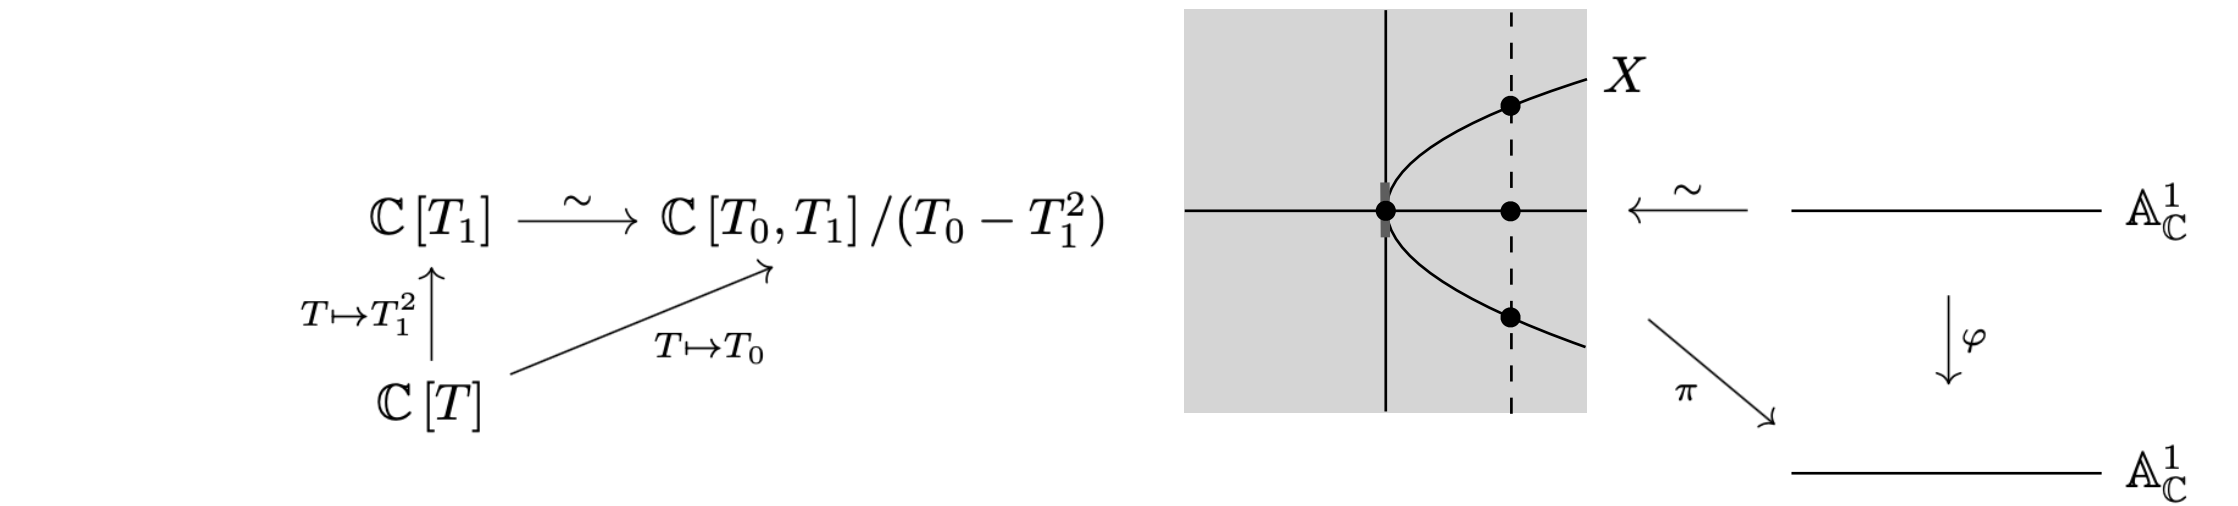
\includegraphics[width = 15cm]{double_cover}
  \end{figure}
  I have drawn the geometry on the right. 
  The isomorphism of $\C[T_1] \iso \C[T_0,T_1]/(T_0 - T_1^2)$
  corresponds to the isomorphism of 
  the parabola $X := V(T_0 - T_1^2)$ to the vertical axis in $\A^2_\C$.
  Our $\ph : \A^1_\C \to \A^1_\C$ then turns into 
  $\pi : X \to \A^1_\C, (t_0, t_1) \mapsto t_0$.
  
  Let $q \in X$. 
  \begin{itemize}
    \item ($\pi(q) = p \in \C$) 
    \begin{cd}
      \spec \ka(q) \ar[r] \ar[d,"\pi"]
      & X \ar[d,"\pi"] 
      & \ka(q) 
      & \C\sqbrkt{T_0,T_1}/(T_0 - T_1^2) \ar[l,"\ev_q"] \\
      \spec \ka(p) \ar[r]
      & \A^1_\C 
      & \C\sqbrkt{T}/(T-p) \ar[u]
      & \C[T] \ar[l,"\ev_p"] \ar[u,"T \mapsto T_0"]
    \end{cd}
    It's easily seen that 
    $\ka(p) \otimes_{\C[T]} \C[T_0,T_1]/(T_0 - T_1^2)
    = \C[T_1]/(p - T_1^2)$.
    So we have $\ka(q) = \C, \ev_q =$ mod $(T_0 - p,T_1 \pm\sqrt{p})$.
    In particular,
    $\pi\inv(0) = \spec \C[T_1]/(T_1)^2$ is a ``double point''. 
    We also say that $0$ is ``ramified''.
    \item ($\pi(q) = p_\infty$)
    \begin{cd}
      \spec \ka(q) \ar[r] \ar[d,"\pi"]
      & X \ar[d,"\pi"] 
      & \ka(q) 
      & \C\sqbrkt{T_0,T_1}/(T_0 - T_1^2) \ar[l,"\ev_q"] \\
      \spec \ka(p_\infty) \ar[r]
      & \A^1_\C 
      & \C(T) \ar[u]
      & \C[T] \ar[l,"\ev_{p_\infty}"] \ar[u,"T \mapsto T_0"]
    \end{cd}
    $\C(T) \otimes_{\C[T]} \C[T_0,T_1] / (T_0 - T_1^2)
    = \C(T_0)[T_1]/(T_0 - T_1^2)$. 
    $\therefore \ka(q) = \C(T)(\sqrt{T}), 
    \ev_q : T_0, T_1 \mapsto T, \sqrt{T}$ is injective. 
  \end{itemize}
\end{eg}

% \begin{eg}[Base Change / ``Enlarging Base Ring'']
%   
%   We saw in the previous example, 
%   that ``traditional solutions'' are precisely $K$-rational points.
%   In number theoretic problems, 
%   it is often convenient to change the set of ``numbers'' you are working with.
%   The framework of schemes accomodates this via 
%   the categorical notion of \emph{fiber products}.
% 
%   Consider the affine variety $X := V(T^2+1) \subs \A^2_\Q$.
%   Then ``over $\Q$ we have no solutions'' means 
%   that the set of $\Q$-rational points $\SCH/\Q(\spec \Q, X)$
%   is empty. 
%   However, given a field extension $K$ of $\Q$,
%   we can consider $K$-rational points of $X$,
%   that is $\SCH/\Q(\spec K, X)$.
%   Indeed, unraveling the definition and using the adjunction,
%   a $K$-rational point $p : \spec K \to X$ 
%   gives : 
%   \begin{cd}
%     \spec K \ar[d] \ar[rd] & & \rightsquigarrow & K & \\
%     \spec \Q & X \ar[l] & & \Q \ar[r] \ar[u] & \Q[T]/(T^2 + 1) \ar[lu]
%   \end{cd}
%   which is precisely a choice of $\la \in K$ such that $\la^2 + 1 = 0$.
%   Instead of checking a point at a time, 
%   we can ``pull $X$ back to $K$'', turning it into a scheme over $K$
%   in the ``least destructive way''.
%   More precisely : 
%   given $X$ over $\Q$, is there a scheme $K \times_\Q X$ over $\Q$
%   such that for all other schemes $Y$ over $K$, 
%   we have \[
%     \SCH/K(Y, K\times_\Q X) \iso \SCH/\Q(Y, X)
%   \]
%   In diagrams, we are looking for : 
%   \begin{cd}
%     & & Y \ar[lld,bend right = 30] \ar[ld, dashed] 
%       \ar[ldd, dashed, bend left = 30] \\
%     \spec K \ar[d] & K\times_\Q X \ar[l] \ar[d] & \\
%     \spec \Q & X \ar[l] &
%   \end{cd}
%   Well, by the adjunction,
%   we are equivalently looking for the dual of this diagram in $\RING$ : 
%   \begin{cd}
%     & & \OO_Y(Y) \\
%     K \ar[rru, bend left = 30] \ar[r] & ? \ar[ru, dashed] & \\
%     \Q \ar[r] \ar[u] & \Q[T]/(1+T^2) \ar[u] \ar[ruu, dashed, bend right = 30] & 
%   \end{cd}
%   This plainly the UP of the tensor product! 
%   So the guy we are looking for is 
%   \[
%     K\times_\Q X := \spec K \otimes_\Q \Q[T]/(1+T^2)
%     = \spec K[T]/(1+T^2)
%   \]
%   And indeed, by the UP of the tensor product : 
%   \[
%     \SCH/K(Y, K\times_\Q X) 
%     \iso K\ALG(K[T]/(1+T^2), \OO_Y(Y))
%     \iso \Q\ALG(\Q[T]/(1+T^2), \OO_Y(Y))
%     \iso \SCH/\Q(Y, X)
%   \]
%   In particular, using $Y = K$, 
%   we see that $K$-rational points of $X$ biject with 
%   $K$-rational points of $K\times_\Q X$.
%   
%   More generally, 
%   given any ring $A$, $A$-algebras $B, C$,
%   we can turn the $A$-scheme $X := \spec C$ into a $B$-scheme 
%   by $B \times_A X := \spec (B \otimes_A C)$.
%   This is called the \emph{base change of $X$ to $B$}.
% 
%   This may seem like a purely algebraic idea, 
%   but here's an example to assure you otherwise. 
%   Consider $\ph : \A^1_\C \to \A^1_\C$ given by $z \mapsto z^2$ geometrically,
%   and $\ph^\flat : \C[T] \to \C[T_0], T \mapsto T_0^2$ algebraically.
%   For a point $p \in \A^1_\C$,
%   the two following situations : 
%   \begin{itemize}
%     \item $p = p_\infty$ the generic point of $\A^1_\C$,
%     then we have the base change as : 
%     \begin{cd}
%       \spec \ka(p) \ar[d] & \ka(p) \times_{\A^1_\C} \A^1_\C 
%         \ar[l] \ar[d]
%         & 
%       \C(T) \ar[r,"T \mapsto T_0^2"] & \C(T_0) \\
%       \A^1_\C & \A^1_\C \ar[l,"\ph"]
%         & 
%       \C[T] \ar[u,"\ev_p"] \ar[r,"T \mapsto T_0^2"{swap}] & \C[T_0] \ar[u]
%     \end{cd}
%     So the base change is nothing more than
%     the generic point of the $\A^1_\C$ on top. 
% 
%     \item $p$ is a closed point corresponding to a $p \in \C$.
%     Then computing the base change of $\ph : \A^1_\C \to \A^1_\C$ to 
%     $\spec \ka(p)$, we get 
%     \begin{cd}
%       \spec \ka(p) \ar[d] & \ka(p) \times_{\A^1_\C} \A^1_\C 
%         \ar[l] \ar[d]
%         & 
%       \C \ar[r] & \C[T_0]/(T_0^2 - p) \\
%       \A^1_\C & \A^1_\C \ar[l,"\ph"]
%         & 
%       \C[T] \ar[u,"\ev_p"] \ar[r,"T \mapsto T_0^2"{swap}] & \C[T_0] \ar[u]
%     \end{cd}
%     So \[
%       \ka(p) \times_{\A^1_\C} \A^1_\C
%       = \begin{cases}
%         \spec \C[T_0]/(T_0 - \sqrt{p}) \times \C[T_0]/(T_0 + \sqrt{p})
%         &\text{ , when } p \neq 0 \\
%         \spec \C[T_0]/(T_0)^2
%         &\text{ , when } p = 0
%       \end{cases}
%     \]
%     
%   \end{itemize}
%   What we have done is nothing more than compute the fiber over points 
%   of the covering $\ph : \A^1 \to \A^1_\C$!
%   You can see that this is a ``branched double cover'' in the sense 
%   that fibers are generically size two, 
%   except for a finite set of points,
%   namely, the generic point and $p = 0$,
%   where the ``2'' appears as the degree of the extension 
%   of residue fields $\C(T) \to \C(T_0), T\mapsto T_0^2$
%   and a ``double point''.
% \end{eg}

\begin{eg}[Infinitesimals]
  
  Let me say a bit more about the ``double point'' in the previous example.
  Consider the following affine schemes over $\C$ : 
  \begin{figure}[H]
    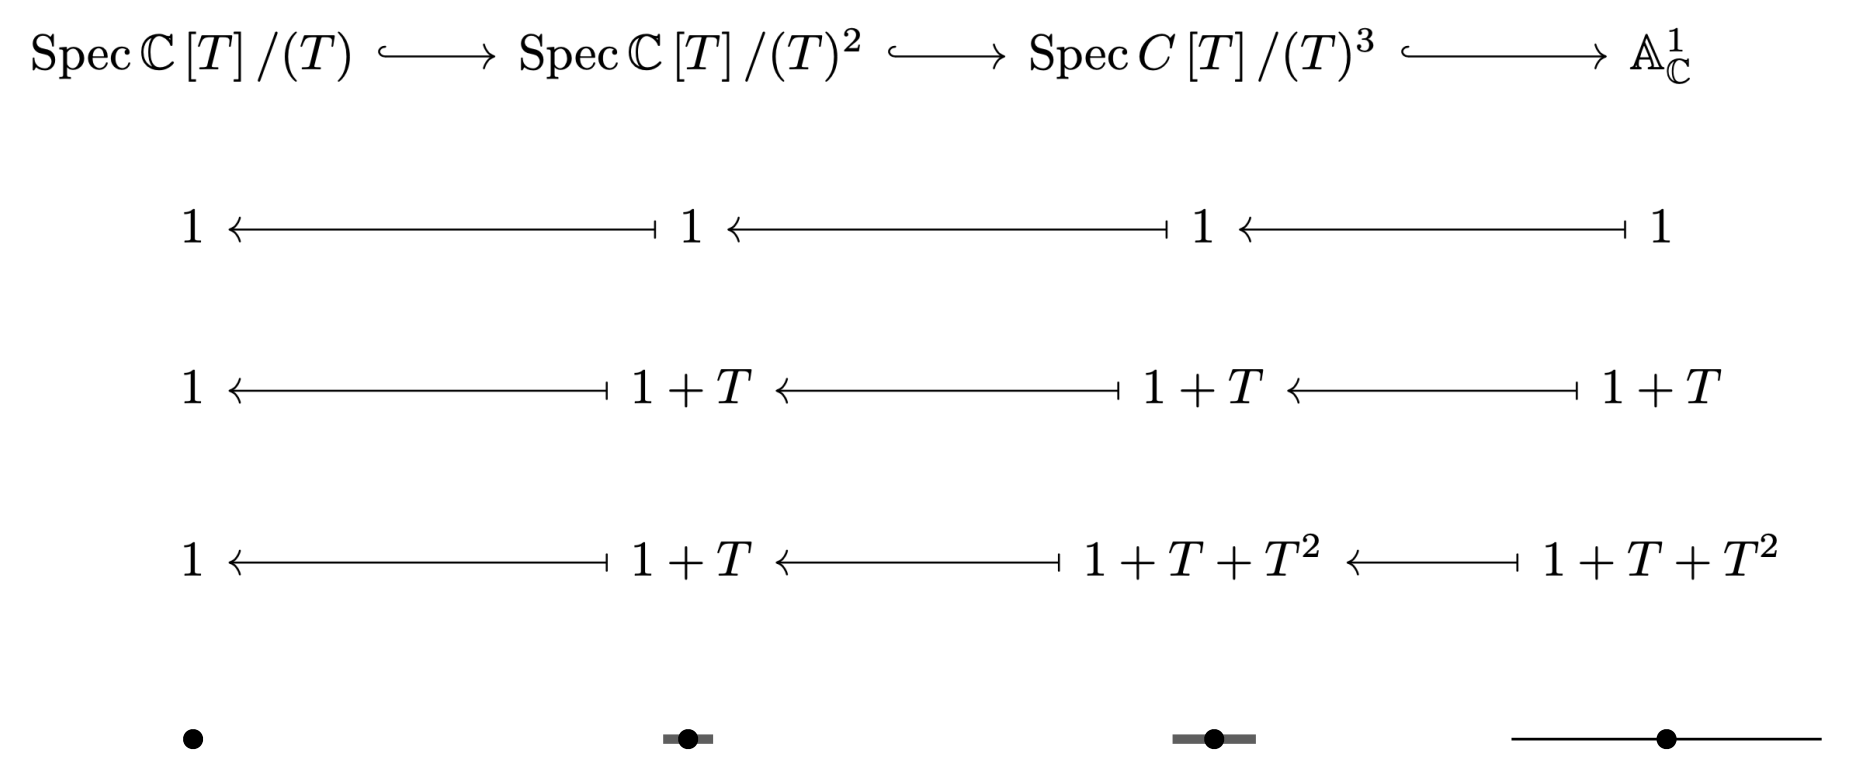
\includegraphics[width = 15cm]{infinitesimal.png}
  \end{figure}
  First, note that 
  the underlying topological spaces of the first 
  three affine schemes are all singletons, 
  corresponding to the point $0 \in \C \hookrightarrow \A^1_\C$.
  
  To demonstrate the ``geometric'' differences between the three,
  consideer the functions $1, 1 + T, 1 + T + T^2 \in \OO_{\A^1_\C}(\A^1_\C)$
  As functions on all of $\A^1_\C$,
  the three functions are clearly different.
  For example, $1$ never vanishes,
  $1 + T$ vanishes at $-1$ whilst 
  $1 + T + T^2$ vanishes at $\om$ primitive third roots of unity, 
  but not at $1$.
  However, pulling back all the way to $\spec \C[T]/(T)$,
  you can no longer tell these three apart.
  This is because ``you only have the data of their values at $0$''.
  But say you only pull back to $\spec \C[T]/(T)^2$.
  Then $1 + T = 1 + T + T^2$ mod $T^2$ but 
  $1 \neq 1 + T$ anymore. 
  Why is this? 
  It's because though all three have the same value at $p = 0$,
  $1$ has derivative $0$ at $p$ whilst 
  $1 + T$ and $1 + T + T^2$ both have derivative $1$ at $p$.
  So the scheme $\spec\C[T]/(T)^2$, 
  though the underlying topological space is the same as 
  the singleton $\spec \C[T]/(T)$,
  it has ``more data than just the point'';
  It also has ``first order infinitesimal data around $0$''.
  Analogously, 
  if you pulled back to $\spec \C[T]/(T)^3$
  you will data at the point, first order data, and second order data.
  We've already seen the general case : 
  nilpotent elements in the ring are precisely 
  the ones that vanish at every point. 
  Their data is not at points but ``infinitesimally around points''.
  For this reason,
  you can think of the three schemes as 
  successive ``first order thickenings'' of the point $0$.

  This suggests a way to think about the derivative of a function 
  $f \in \C[T] = \OO_{\A^1_\C}(\A^1_\C)$ at $0$ : 
  simply look at $f - \ev_0(f)$ in $\C[T]/(T)^2$. 
  This is the same as 
  $\C[T] \to (T)/(T)^2, f \mapsto f - \ev_0(f)$.
  It is easily seen that $(T)/(T)^2$ is a one dimensional vector space over 
  $\ka(0) = \C$.
  This is precisely the \textit{cotangent space at $0$}.

  Let me walk through this in the more elaborate example of 
  the ramified double cover $\pi : X = V(T_0 - T_1^2) \to \A^1_\C$.
  Let $q \in X$ be a closed point.
  Define 
  \begin{align*}
    T_q^* X &:= I(q)/I(q)^2 \in \ka(q)\VEC \\
    (\De f)_q &:= f - \ev_q(f) \\
    (df)_q &:= \text{ image of $(\De f)_q$ in $T_q^* X$}
  \end{align*}
  In particular, $I(q) = (T_0 - T_0(q), T_1 - T_1(q))
  = ((\De T_0)_q, (\De T_1)_q)$, 
  so \[
    T_q^* X = \C (dT_0)_q + \C (dT_1)_q
  \]
  But since we are on the parabola, 
  $(\De T_0)_q = T_0 - \ev_q(T_0) 
  = T_1^2 - \ev_q(T_1)^2 = (T_1 + \ev_q(T_1)) (\De T_1)_q$,
  so $(dT_0)_q = 2 \ev_q(T_1) (dT_1)_q$ in the cotangent space at $q$.
  \[
    \therefore T_q^* X = \frac{\C (dT_0)_q \oplus \C (dT_1)_q}
    {\C\brkt{(dT_0)_q - 2 \ev_q(T_1) (dT_1)_q}} 
    = \frac{T_q^* \A^2_\C}{\C\brkt{(dT_0)_q - 2 \ev_q(T_1) (dT_1)_q}}
  \]
  where we secretly computed $T^*_q\A^2_\C$ with basis $(dT_0)_q, (dT_1)_q$.
  This quotient is just the algebraic side of the 
  geometric fact that 
  ``moving along $V(T_0 - T_1^2)$ doesn't change $T_0 - T_1^2$''.
  Below, I have drawn a picture of the first order neighbourhood of 
  some $q \in X$ and $(0,0) \in X$.
  \begin{figure}[H]
    \centering
    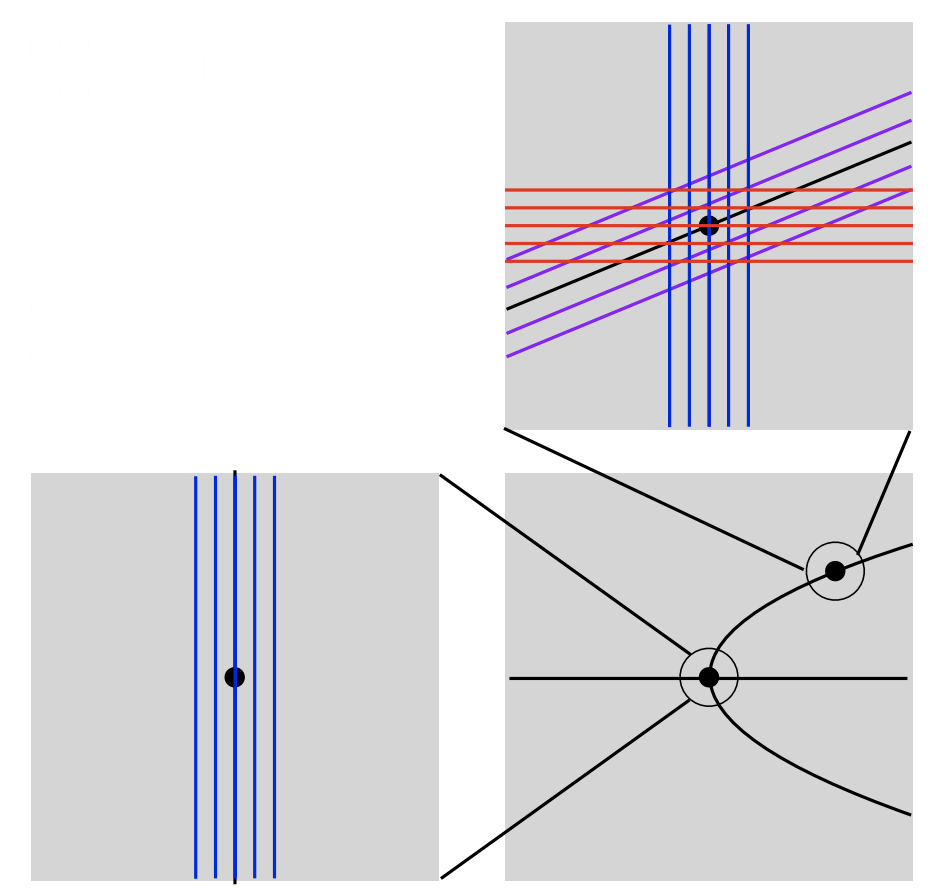
\includegraphics[width = 8cm]{cotangent.png}
  \end{figure}
  The blue, red and purple lines are the level sets of 
  $(dT_0)_q, (dT_1)_q, d(T_0 - T_1^2)_q = (dT_0)_q - 2\ev_q(T_1)(dT_1)_q$
  respectively. 

  Another nice thing about this definition of 
  cotangent space is that it's easy to see how this interacts with morphisms.
  To demonstrate, let $p = \pi(q)$. 
  Then \[
    I(p) \to I(q), (\De T)_p \mapsto (\De T_0)_q 
  \]
  which by UP of quotients of modules, 
  descends down to 
  \[
    T_p^* \A^1_\C \to T_q^* X, (dT)_p \mapsto (dT_0)_q
  \]
  In particular, $T_0^* \A^1_\C \to T_{(0,0)}^* X$ is the zero morphism. 
  This is just the geometric fact that 
  in the first order neighbourhood of $X$ around $(0,0)$, 
  there's no way to move that causes 
  a change in the coordinate function $T_0$.
  In other words, the ``tangent space of $X$ at $(0,0)$ is vertical''.

  % The cool thing is you can use the first order thickening 
  % $\spec \C[T]/(T)^2$ to give a notion of tangent space for varieties.
  % Let us consider the branched double cover 
  % $\A^1_\C \to \A^1_\C, z \mapsto z^2$ again. 
  % To get a better view of what's going on,
  % let us rewrite the ring morphism 
  % $\C[T] \to \C[T_0], T\mapsto T_0^2$ as 
  % $\C[T] \to \C[T_0,T_1]/(T_0 - T_1^2), T \mapsto T_0$.
  % By the adjunction, this rewriting corresponds to 
  % factoring the branched double cover through 
  % an closed embedding to $\A^2_\C$ : 
  % \begin{cd}
  %   \C\sqbrkt{T_0} = \frac{\C\sqbrkt{T_0,T_1}}{(T_0 - T_1^2)}
  %   & \C\sqbrkt{T_0,T_1} \ar[l]
  %   & \A^1_\C \ar[r,hook] \ar[rd,"\ph"{swap}] 
  %   & V(T_0 - T_1^2)\subs\A^2_\C \ar[d,"\pi"] \\
  %   & \C\sqbrkt{T} \ar[ul,"T\mapsto T_0"] \ar[u,"T\mapsto T_0"{swap}] 
  %   &
  %   & \A^1_\C
  % \end{cd}
  % (Draw parabola boi.)
  % First, for a $\C$-rational point $p \in \A^1_\C$,
  % you can consider all the different ways of 
  % extending the embedding $\spec \ka(p) \to \A^1_\C$
  % to a first order thickening 
  % $\spec \ka(p) \to \spec\ka(p)[\ep]/(\ep)^2$.
  % Diagrammatically,
  % \begin{cd}
  %   \spec \ka(p) \ar[r] \ar[d]
  %   & \A^1_\C \ar[d]
  %   & \ka(p)
  %   & \C[T] \ar[l,"\ev_p"{swap}] \ar[ld,dashed,"\de_v"]\\
  %   \spec \ka(p)[\ep]/(\ep)^2 \ar[r] \ar[ru,dashed,"v"]
  %   & \spec \C 
  %   & \ka(p)[\ep]/(\ep)^2 \ar[u] 
  %   & \C \ar[l] \ar[u]
  % \end{cd} 
  % By the UP of $\C[T]$,
  % such $\de_v$ is uniquely determined by where it sends $T$.
  % So we see that for every $\la \in \C$,
  % we have a lift $v_\la$ corresponding to $\de_\la(T) = \ev_p(T) + \la \ep$.
  % You can think of this as saying 
  % ``there is one dimensional amount of first order infinitesimal space 
  % around $p \in \A^1_\C$''.
  % Hence, 
  % it is not unreasonable to define \[
  %   T_p\A^1_\C := \set{\text{ lifts of } \spec\ka(p)[\ep]/(\ep)^2}
  % \]
  % This is somewhat analogous to the curves definition of 
  % tangent space for manifolds.
% 
  % Now the interesting question is this : 
  % at which $K$-rational points $p \in V(T_0 - T_1^2)$ 
  % is the projection $\pi$ a ``immersion'' or ``submersion''?
  % That is to say,
  % given a tangent vector $v_\la \in T_{\pi(p)}\A^1_\C$,
  % when can you lift $v_\la$ to a tangent vector at $p$,
  % and if so, when is it unique? 
  % Let's compute.
  % The setup is this : 
  % \begin{cd}
  %   \spec \ka(p) \ar[r] \ar[d]
  %   & V(T_0 - T_1^2) \ar[d]
  %   & \ka(p)
  %   & \C[T_0,T_1]/(T_0-T_1^2) \ar[l,"\ev_p"{swap}] 
  %     \ar[ld,dashed,"\bar{\de_\la}"]\\
  %   \spec \ka(p)[\ep]/(\ep)^2 \ar[r,"v_\la"] \ar[ru,dashed,"\bar{v_\la}"]
  %   & \A^1_\C
  %   & \ka(p)[\ep]/(\ep)^2 \ar[u] 
  %   & \C[T] \ar[l,"\de_\la"] \ar[u]
  % \end{cd} 
  % where $\de_\la(f) = \ev_p(f) + \la\ep$ for some $\la \in \C$.
  % Again, such $\de_v$ is determined by where $T_0$ and $T_1$ goes.
  % Let $\de_v(T_0) = a + b\ep, \de_v(T_1) = c + d\ep$.
  % First of all, we have 
  % \[ a = \ev_p(T_0), c = \ev_p(T_1) \]
  % Then there's also 
  % \[
  %   \ev_p(T) + \la \ep 
  %   = \de_\la(T)
  %   = \bar{\de_\la}(T_0)
  %   = \ev_p(T_0) + b \ep
  %   = \ev_p(T) + b \ep
  % \]
  % so $b = \la$.
  % Finally, $T_0 = T_1^2$ implies 
  % \[
  %   \la = 2\ev_p(T_1) d
  % \]
  % The only free variable left is $d$.
  % We have two cases : 
  % \begin{itemize}
  %   \item ($\ev_p(T_1) \neq 0$) Then $d$ is determined uniquely.
  %   In this case we have a unique lift $\bar{v_\la}$.
  %   \item ($\ev_p(T_1) = 0$)
  %   We have $\la = 0$ and $d$ can be anything. 
  %   So if $\la \neq 0$, we dont have any lift and 
  %   if $\la = 0$, we have a lift $\bar{v_\la}$ for every $\la \in \C$.
  % \end{itemize}
  % We have just shown that 
  % other than the point $(0,0)$,
  % the projection $\pi$ gives an isomorphism of tangent spaces
  % and at $(0,0)$,
  % the kernel of the map on tangent spaces is one dimensional.
  % But is trivial by the picture.
  % We have just confirmed our intuition that 
  % at $(0,0)$, the tangent space is vertical and so dies under
  % the projection.
  % This corresponds precisely with 
  % the fact that the fiber at $p = 0 \in \A^1_\C$
  % is a double point. 
  % It is this ``extra first order space'' that allows us 
  % to lift tangent vectors.

\end{eg}

\begin{eg}[Algebraic Number Theory]

  I said at the beginning of the article that 
  generality of schemes was made to unify number theory with geometry so
  let me demonstrate with the following example.
  
  One of the main problems that tackled in algebraic number theory is 
  whether a prime $p \in \Z$ stays prime in a ring extension of $\Z$,
  like $\Z[i]$.
  This is an entirely geometric problem. 
  We have already seen that points of $\spec \Z$ are primes 
  (and a generic point). 
  This is also true for $\Z[i]$ : 
  Since $\Z[i]$ is PID, 
  non-injective maps $\Z[i] \to K$ into fields have 
  kernels generated by prime elements
  and conversely, prime elements are irreducible 
  so $\Z[i]$ PID implies quotienting by them give fields. 
  There is, again, a generic point $q_\infty$
  where $\ev_{q_\infty} : \Z[i] \to \ka(q_\infty) = \Q(i)$.

  Let $p \in \spec \Z$.
  We are interested in $q \in \spec \Z[i]$ that divide $p$.
  Elementarily, this means $(p) \subs (q)$ as ideals in $\Z[i]$.
  Algebraically, this is nothing more than saying we have a factoring : 
  \begin{cd}
    \ka(q) & \Z[i] \ar[l,"\ev_q"] \\
    \ka(p) \ar[u, dashed] & \Z \ar[l,"\ev_p"] \ar[u]
  \end{cd}
  in other words, \textit{$q$ is in the fiber over $p$}.
  Hence the terminology ``$q$ is a prime lying over $p$''
  used in algebraic number theory. 
  In fact, we have something stronger : 
  for $e \in \N$, 
  \begin{align*}
    q^{e + 1} \mid p \iff 
    \spec \Z[i]/q^{e+1} \hookrightarrow \pi\inv(p)
  \end{align*}
  ``the $e$-th order neighbourhood of $q$ is in the fiber over $p$''. 
  Using fiber products, this is but a computation. 
  \begin{itemize}
    \item Let $p \in \spec \Z$ be not the generic point. 
    Then we have : 
    \begin{cd}
      \spec \F_p[T]/(1 + T^2) = \pi\inv(p) \ar[d] \ar[r]
      & \spec \Z[i] \ar[d,"\pi"] \\
      \spec \F_p \ar[r]
      & \spec \Z
    \end{cd}
    So \[
      \pi\inv(p) = \begin{cases}
        \spec \frac{\F_p[T]}{(\sqrt{-1} + T)} \times 
        \spec \frac{\F_p[T]}{(-\sqrt{-1} + T)}
        &\text{ , when there are two square roots of $-1$ mod $p$} \\
        \spec \F_p[T]/(1+T)^2 
        &\text{ , when $p = 2$} \\
        \spec \F_p[T]/(1+T^2) 
        \text{ singleton}
        &\text{ , when $-1$ is not a quadratic residue mod $p$} 
      \end{cases}
    \]
    \item For completeness sake, let's also calculate the fiber of 
    the generic point $p_\infty \in \spec \Z$.
    \begin{cd}
      \spec \Q(i) = \pi\inv(p_\infty) \ar[d] \ar[r]
      & \spec \Z[i] \ar[d,"\pi"] \\
      \spec \Q = \spec \ka(p_\infty) \ar[r]
      & \spec \Z
    \end{cd}
    So the fiber over generic point of $\spec \Z$
    is just the generic point of $\spec \Z[i]$.
  \end{itemize}
  What's cool is that this looks 
  exactly like the branched double cover $\A^1_\C \to \A^1_\C, z \mapsto z^2$. 
  \begin{itemize}
    \item for $-1$ a quadratic residue mod $p$ and two distinct roots,
    the distinct roots correspond to the fiber over $p$ having two points.
    I think of this as why they call these primes \emph{split}.
    An example is $(5) = (2 - i)(2 + i)$ in $\Z[i]$.

    These split primes $q$ looks like $(p,\la \pm i)$
    where $\la \in \Z$ is a square root of $-1$ mod $p$.
    \item The fiber over $p = 2$ is a double point,
    i.e. this is a ``branch point'' of the cover,
    hence the terminology \emph{ramified primes}.
    In particular, $(2) = (1+i)^2$ in $\Z[i]$.
    \item For $-1$ not quadratic residue mod $p$,
    the fiber is a single point and 
    the pullback of residue fields $\F_p \to \F_p[T]/(1+T^2)$
    is a degree two extension.
    These are the \emph{inert primes}.
    An example is $(3)$ in $\Z[i]$.
    \item For the generic point $p_\infty$,
    the pullback on residue fields $\Q \to \Q(i)$ is also a 
    degree two extension.
  \end{itemize}
  Now, I know you could figured this out by playing around with
  the Euclidean norm,
  but I find this clearer.
  The framework systematically accounts for the different cases,
  treating them on an equal level and 
  you can see why whether $-1$ is a quadratic residue is relevant. 
  Also, 
  wouldn't you agree that 
  seeing fibers of a branched double cover
  is nicer than playing around with some numbers? 

  Another nice thing is that the earlier discussion of cotangent spaces 
  generalize to here, 
  since we only used the notion of the ideal of a point. 
  Let's compute $T^*_q\spec \Z[i]$ and its relation to $T^*_p\spec\Z$
  where $p = \pi(q)$.
  
  First, for $p \in \spec\Z$ (non-generic), we have
  $T_p^*\Z = I(p)/I(p)^2 = (p)/(p)^2 = \F_p (dp)_p$,
  a one dimensional vector space over $\ka(p) = \F_p$.
  This also suggests one should be seeing $\spec \Z$
  as a ``curve'', like $\A^1_\C$ and the parabola $V(T_0 - T_1^2)$.
  For $q \in \spec\Z[i]$ (non-generic), 
  we case on whether $p$ is inert : 
  \begin{itemize}
    \item (\textit{$p$ inert}) 
    We have $I(q) = (q) = (p)$, so
    \begin{cd}
      T_p^*\spec\Z \otimes_{\F_p} \F_{p^2} \ar[r,"\sim"] & T_q^*\spec\Z[i] \\
      (p)/(p)^2 \ar[r,"\sim"] & (p)/(p)^2
    \end{cd}
    We had to extend scalars here because the pullback of residue fields
    $\ka(p) \to \ka(q)$ is a non-trivial extension. 
    This did not appear in our computation of cotangent spaces in 
    the ramified double cover because all finite extensions of $\C$ are trivial
    by $\C$ algebraically closed. 
    \item (\textit{$p$ not inert})
    We have $I(q) = (p, \la + i)$ where $\la^2 + 1 = 0$ mod $p$,
    and $\ka(q) = \ka(p) = \F_p$.
    Projecting into the cotangent space at $q$, we get : 
    \[ 
      T_q^*\spec\Z[i] = \F_p(dp)_q + \F_pd(\la + i)_q 
    \]
    But $np = 1 + \la^2 = (\la - i)(\la + i)$ for some $n \in \Z$ 
    implies $n (dp)_q = (\la - i) d(\la+i)_q$.
    So for $p \neq 2$,
    $\la - i \neq 0 \in \ka(q)$ gives 
    \[
      T_p^*\spec\Z \iso T_q^*\spec\Z[i]
    \]
    as $\F_p$ vector spaces.

    For $p = 2$, $q = (1 + i)$,
    $2 = (1 - i)(1 + i)$ gives $(d2)_q = (1 - i) d(1+i)_q = 0$ 
    since $i = 1$ in $\ka(q)$.
    Thus, 
    \[
      T_2^*\spec\Z \overset{0}{\to} T_{(1+i)}^*\spec\Z[i]
    \]
  \end{itemize}
  The above is, again, complete analogous to the 
  ramified double cover where the pullback of cotangent spaces are 
  isomorphisms everywhere except at ramified points. 
  You can thus think of the ``tangent space of $\spec\Z[i]$''
  as being ``vertical over $2 \in \spec\Z$''.
\end{eg}

\begin{eg}[Power Series and $p$-adics]
  
  Recall that given a field $K$,
  you can see $\spec K[T]/(T)^{n+1}$ geometrically as 
  $n$-th order neighbourhood of $0 \in \A^1_K$,
  corresponding algebraically to the fact that 
  functions are determined up to the first $n$ derivatives.
  It's pretty natural then to want to consider 
  the union of these infinitesimal neighbourhoods,
  which is sometimes called the \emph{formal disk around $0$}.
  What ring should this correspond to? 
  Well, ``the ring of functions defined 
  on all infinitesimal neighbourhoods of $0$'',
  i.e. \emph{power series}.
  \begin{cd}
    & 
    & \spec K\llbracket T \rrbracket 
    & & \\
    \spec K[T]/(T) \ar[r] \ar[rru, bend left = 10]
    & \spec K[T]/(T)^2 \ar[r] \ar[ru]
    & \cdots \ar[r] \ar[u]
    & \spec K[T]/(T)^{n+1} \ar[r] \ar[lu]
    & \cdots \ar[llu, bend right = 10]
  \end{cd} 
  Hence the definition of $K\llbracket T \rrbracket$ as 
  the inverse limit of $K[T]/(T)^{n+1}$.
  \begin{cd}
    & 
    & K\llbracket T \rrbracket 
      \ar[dll,bend right = 10]
      \ar[dl] \ar[d] \ar[dr]
      \ar[drr, bend left = 10]
    & & \\
    K[T]/(T) \ar[r] 
    & K[T]/(T)^2 \ar[r] 
    & \cdots \ar[r] 
    & K[T]/(T)^{n+1} \ar[r] 
    & \cdots 
  \end{cd} 
  The ring $\C((T)) = \text{Frac }\C\llbracket T\rrbracket$ of
  formal laurent series with finite pole at $0$
  corresponds geometrically to the punctured formal disk around $0$.

  Now, we can play the same game with $\spec \Z$.
  Let $p \in \spec \Z$ be a point corresponding to a prime $p \in \Z$.
  Then we have the following geometric picture : 
  \begin{cd}
    & 
    & \spec\,?
    & & \\
    \spec \Z/(p) \ar[r] \ar[rru, bend left = 10]
    & \spec \Z/(p)^2 \ar[r] \ar[ru]
    & \cdots \ar[r] \ar[u]
    & \spec \Z/(p)^{n+1} \ar[r] \ar[lu]
    & \cdots \ar[llu, bend right = 10]
  \end{cd} 
  where the ring corresponding to 
  the union of infinitesimal neighbourhoods of $p$
  is none other than $\Z_p$ the $p$-adic integers.
  Then $\Q_p = \text{Frac }\Z_p$ is of course 
  the ring of functions on the punctured formal disk around $p$.
  I like to think of this as the reason for the prefix 
  ``local'' in local class field theory. 
\end{eg}

\section{Locally Ringed $\spec$}

\begin{rmk}
  Now that we're motivated by some exotic examples,
  let us complete the construction of $\spec$ and prove the adjunction.

  A pretopology carries all the data of the topology it generates. 
  In particular, on a topological space $X$,
  given a pretopology $B \subs \tau_X$ generating $\tau_X$,
  we have for every open $U$, 
  $U$ is the union of all basis opens $V \in B$ inside it.
  Then for a sheaf of rings $\OO$ on $X$, 
  \[
    \OO(U) = \LIM_{U \sups V \in B} \OO(V)
  \]
  which is just saying ``a function on $U$ is the equivalent to 
  a compatible system of functions on basis opens inside $U$''.
  This says the sheaf $\OO$ is completely determined by 
  its values on the pretopology $B$.
  This suggests if we have the data of a sheaf on $B$,
  then we can extend it to a sheaf on all opens of $X$. 
  Here's the precise statement.
  
\end{rmk}

\begin{lem}[Sheaf on Basis]
  
  Let $X \in \TOP$, $B \subs \tau_X$ a pretopology generating $\tau_X$.
  A \emph{sheaf of rings on $B$} is defined by 
  the following pieces of data : 
  \begin{enumerate}
    \item a functor $\OO : B\op \to \RING$, assigning rings to 
    opens in the pretopology, together with restriction morphisms along 
    inclusions. 
    \item (Unique Gluing)
    Let $U \in B$, $\UU \subs B$ with $\bigcup_{V \in \UU} V = U$
    and $(f_V) \in \prod_{V \in \UU} \OO(V)$ a collection of functions
    such that for all $V, V_1 \in \UU$,
    $\fall{W}{V} f_V = \fall{W}{V_1} f_{V_1}$ 
    on every basis open $W \subs U \cap V$.
    Then there exists a unique $f \in \OO(U)$ such that
    for all $V \in \UU$, $\fall{V}{U} f = f_V$.
  \end{enumerate}

  Let $\OO$ be a sheaf of rings on $B$.
  For every $U \in \tau_X$,
  define \[
    \OO^e(U) := \LIM_{U\sups V \in B} \OO(V)
  \]
  Then $\OO^e$ is a sheaf of rings on $\tau_X$ 
  which agrees with $\OO$ on $B$.
\end{lem}
\begin{proof}
  Straightforward but lengthy.  
  All the intuition is in the statement. 
\end{proof}

\begin{rmk}
  Thus, to define the structure sheaf of $\spec A$,
  we only need to define it on the basic opens $U \in D(A)$.
  We know already that for $U = D(f)$, $U = \spec A_f$,
  which indicates we should define $\OO(U) := A_f$.
  Again, using wishful thinking, 
  assuming $\spec : \RING\op \to \LRSP$ satisfies the adjunction,
  we actually have something stronger. 
  \[
    \LRSP(X,D(f)) \overset{(1)}{\iso} \RING(A_f,\OO_X(X)) 
    \overset{(2)}{\iso} \LRSP(X,\spec A_f)
  \]
  where $D(f)$ is given the obvious locally ringed space structure of 
  any open subspace and the justifications of the isomorphisms are : 
  \begin{enumerate}
    \item Given a morphism $\ph : X \to \spec A$,
    $\ph X \subs D(f)$ if and only if 
    $\ph^\flat_{\spec A}(f) \in \OO_X(X)^\times$,
    which is equivalent a factoring of the global pullback 
    \begin{cd}
      \OO_X(X) & A_f \ar[l,dashed] \\
      A \ar[u,"\ph^\flat_{\spec A}"] \ar[ur]
    \end{cd}
    \item the adjunction.
  \end{enumerate}
  Using this bijection on $X = D(f)$ and $\spec A_f$,
  one obtains an isomorphism $D(f) \iso \spec A_f$ as locally ringed spaces.
  (i.e. Yoneda's lemma.)

  However, 
  there may be $g \neq f$ with $D(g) = D(f)$,
  which leads to a choice if we define $\OO(U)$ this way. 
  (Exercise : find an example of $f \neq g \in A$, with $D(f) = D(g)$.)
  To avoid this, note that 
  $U = \spec S_U\inv A$ where $S_U := \set{f \in A \st U \subs D(f)}$,
  giving us the following definition. 
\end{rmk}

\begin{prop}[Structure Sheaf of $\spec A$]
  
  Let $A \in \RING$.
  For $U \in D(A)$, 
  define \[
    \OO_{\spec A}(U) := S_U\inv A
  \]
  where $S_U = \set{f \in A \st U \subs D(f)}$ as mentioned before. 
  In particular, note that $\OO_{\spec A}(\spec A) = A$ by the Nullstellensatz.
  Then
  \begin{enumerate}
    \item For any $f \in A$ and $U = D(f)$,
    $\OO_{\spec A}(U) \iso A_f$ canonically as $A$-algebras. 
    \item $\OO_{\spec A}$ is a sheaf of rings on $D(A)$,
    and hence extends to a sheaf of rings on $\spec A$.
  \end{enumerate} 
\end{prop}
\begin{proof}
  $(1)$
  I claim that $S_U\inv A$ has the UP of $A_f$ as an $A$-algebra,
  and we prove it geometrically. 
  Let $\ph^\flat : A \to B$ be a ring morphism where 
  $\ph^\flat(f) \in B^\times$.
  Let $\ph^\tau : \spec B \to \spec A$ be 
  the corresponding topological morphism.
  Then $\ph^\flat(f) \in B^\times$ says 
  ${\ph^\tau}\inv D(f) = D(\ph^\flat(f)) = \spec B$. 
  So for any $g \in S_U$, 
  we must also have ${\ph^\tau}\inv D(g) = D(\ph^\flat(g)) = \spec B$.
  But by the Nullstellensatz, this implies $\ph^\flat(g) \in B^\times$,
  so by the UP of $S_U\inv A$, we are done. 

  $(2)$
  Let $U \in D(A)$, $\UU \subs D(A)$, $U = \bigcup_{V \in \UU} V$,
  $(f_V) \in \prod_{V \in \UU} \OO_{\spec A}(V)$ such that 
  for all $V, V_1 \in \UU$ and basic open $W \subs V \cap V_1$,
  we have $\fall{W}{V}f_V = \fall{W}{V_1} f_{V_1}$.
  Note that first, since $U = \spec S_U\inv A$ and 
  restriction of basic opens to $U$ is still basic,
  we can WLOG assume $U = \spec A$. 

  Here's a crazy reduction. 
  Suppose for a moment, 
  for any finite subcover $\UU_0 \subs \UU$,
  we have a unique $f_{\UU_0} \in \OO(U)$ that 
  agree with $f_V$ on $V \in \UU_0$.
  Then since $U = \spec A$ is \emph{quasi-compact},
  we have a finite subcover $\UU_0$ and such $f_{\UU_0}$.
  Furthermore, 
  for any $V \in \UU$, $f_{\UU_0} = f_{\UU_0 \cup \set{V}}$ by 
  uniqueness of $f_{\UU_0}$ on $\UU_0$ so
  \[
    \fall{V}{} f_{\UU_0} = \fall{V}{} f_{\UU_0 \cup \set{V}} = f_V
  \]
  So $f_{\UU_0}$ actually agrees with $f_V$ on all $V \in \UU$.
  Furthermore, it is unique, again by uniqueness on $\UU_0$.
  Thus, it suffices to do the case of \emph{$\UU$ finite}.


  The naive idea is this : 
  if each $f_V = g_V / h_V$ with $V = D(h_V)$,
  then ``agreeing on intersections'' \emph{should} mean 
  $g_V h_W = g_W h_V \in \OO(U) = A$.
  We can then use a partition of unity $1 = \dsum{V \in \UU}{} \la_V h_V$
  to patch : \[
    f_V = \frac{g_V}{h_V}
    = \frac{\dsum{W \in \UU}{} \la_W g_V h_W}{h_V}
    = \frac{\dsum{W \in \UU }{} \la_W g_W h_V}{h_V}
    = \frac{\dsum{W \in \UU}{} \la_W g_W}{1}
  \]
  So $f := \dsum{W \in \UU}{} \la_W g_W \in A = \OO_{\spec A}(U)$ 
  is the guy we want. 
  This is even unique since if we have another such $f_1$,
  then $f/1 = f_1 / 1 \in \OO(V) \iso A_{h_V}$ implies
  the existence of $N_V \in \N$ such that $(f - f_1) h_V^{N_V} = 0$.
  By \emph{finiteness of $\UU$},
  we can pick a single $N \in \N$ with 
  $(f - f_1) h_V^N = 0$ for all $V \in \UU$.
  Then using another partition of unity $1 = \dsum{V \in \UU}{} \mu_V h_V^N$,
  we have \[
    f - f_1 = \dsum{V \in \UU}{} \mu_V (f - f_1) h_V^N = 0
  \]
  It thus suffices to write for all $V \in \UU$,
  $f_V = g_V / h_V$ such that for all $W \in \UU$, $g_V h_W = g_W h_V$.

  Well, for each $V \in \UU$, let $h_V \in A$ with $V = D(h_V)$.
  Then $f_V = g_V / h_V^{n_V}$.
  Since $D(h_V) = D(h_V^{n_V})$, WLOG $f_V = g_V / h_V$ with $V = D(h_V)$
  Now, since $f_V$ and $f_W$ agree on $V \cap W = D(h_V h_W)$,
  we have $g_V h_W / h_V h_W = \fall{V\cap W}{} g_V / h_V
  = \fall{V \cap W}{} g_W / h_W = g_W h_V / h_V h_W$
  and so the existence of $n(V,W) \in \N$ such that
  \[
    (g_V h_W - g_W h_V) (h_V h_W)^{n(V,W)} = 0
  \]
  Smashing it again with \emph{finiteness of $\UU$},
  we can choose a single $N \in \N$ such that 
  \[
    (g_V h_W - g_W h_V) (h_V h_W)^N = 0
  \]
  for \emph{all} $V, W \in \UU$.
  Then, since $g_V / h_V = g_V h_V^{N} / h_V^{N+1} $
  and $D(h_V) = D(h_V^{N+1})$,
  we can WLOG $f_V = g_V / h_V$ with $V = D(h_V)$ and \[
    g_V h_W - g_W h_V = 0
  \]
  as desired, finishing the proof.
\end{proof}

\begin{rmk}
  We are ready to define $\spec : \RING\op \to \LRSP$.
\end{rmk}

\begin{prop}[Locally Ringed $\spec$]
  
  Let $A \in \RING$.
  \begin{itemize}
    \item (Jointly Surjective Evaluation)
    Let $p \in \spec A$.
    For any open neighbourhood $U$ of $p$,
    there exists a smaller basic open neighbourhood $U_0$ of $p$.
    By the UP of localization, 
    there a unique dashed ring morphism 
    \begin{cd}
      A \ar[r,"\ev_p"] \ar[d]& \ka(p) \\
      \OO(U_0) \ar[ru,dashed] & 
    \end{cd}
    Define \[
      (\ev_p)_U := \OO(U) \to \OO(U_0) \to \ka(p)
    \]
    Then this ring morphism is independent of the choice of $\UU_0$
    and for every $\la \in \ka(p)$,
    there exists some function $f$ on some open neighbourhood $U$ of $p$
    such that $(\ev_p)_U(f) = \la$.
    \item (Invertible on Open Support)
    For a function $f$ on any open $U$ of $\spec A$,
    its support $D(f)$ is open and $f$ is invertible on $D(f)$.
  \end{itemize}
  The above data makes $\spec A$ with its structure sheaf a 
  locally ringed space. 

  Now let $\ph^\bot : A \to B$ be a ring morphism.
  We define the morphism of locally ringed spaces 
  $\ph : \spec B \to \spec A$ as follows : 
  \begin{itemize}
    \item (Underlying Topological Morphism) 
    $\ph^\tau : \spec B \to \spec A$ corresponding to $\ph^\bot$.
    \item (Pullback of Functions)
    For an open $U$ of $\spec A$, 
    $U = \bigcup \set{U_0 \in D(A) \st U_0 \subs U}$.
    This implies 
    ${\ph^\tau}\inv U = \bigcup \set{{\ph^\tau}\inv U_0 \st U_0 \subs U}$,
    where the ${\ph^\tau}\inv U_0$ are also basic opens. 
    Since $\ph^\bot S_{U_0} \subs S_{{\ph^\tau}\inv U_0}$,
    by the UP of localization, we have a unique ring morphism 
    $\ph^\flat_{U_0}$ such that : 
    \begin{cd}
      B \ar[d] & A \ar[l,"\ph^\bot"{swap}] \ar[d] \\
      \OO_{\spec B}({\ph^\tau}\inv U_0) & 
        \OO_{\spec A}(U_0) \ar[l,"\ph^\flat_{U_0}"]
    \end{cd}
    Using unique gluing of $\OO_{\spec B}$ on ${\ph^\tau}\inv U$,
    we have a unique ring morphism $\ph^\flat_U$ such that :
    \begin{cd}
      \OO_{\spec B}({\ph^\tau}\inv U) \ar[d] & 
        \OO_{\spec A}(U) \ar[l,"\ph^\flat_U"{swap}] \ar[d] \\
      \OO_{\spec B}({\ph^\tau}\inv U_0) & 
        \OO_{\spec A}(U_0) \ar[l,"\ph^\flat_{U_0}"]
    \end{cd}
    Then for any inclusion of opens $V \subs U$,
    we have pulling back commuting with restriction : 
    \begin{cd}
      \OO_{\spec B}({\ph^\tau}\inv U) \ar[d] & 
        \OO_{\spec A}(U) \ar[l,"\ph^\flat_U"{swap}] \ar[d] \\
      \OO_{\spec B}({\ph^\tau}\inv V) & 
        \OO_{\spec A}(V) \ar[l,"\ph^\flat_{V}"]
    \end{cd}
    \item (Pullback of Residue Fields)
    Already defined. 
    \item (Commuting Evaluation and Pullback of Residue Fields)
    We have for any point $p \in \spec B$,
    \begin{cd}
      \OO_{\spec B}\circ{\ph^\tau}\inv \ar[d,"\ev_x"{swap}] & 
      \OO_{\spec A} \ar[l,"\ph^\flat"{swap}] \ar[d,"\ev_{\ph(x)}"] \\
      \ka(p) & \ar[l,"\ph^\ka_p"] \ka(\ph(p))
    \end{cd}
  \end{itemize}
  The above data turns $\spec$ into a functor $\RING\op \to \LRSP$.

\end{prop}
\begin{proof}
  
  \textit{(Jointly Surjective Evaluation)}
  For independence of choice of $U_0$, 
  let $U_1$ be another basic open neighbourhood of $p$ contained in $U$.
  Then by the UP of localization, we have the following commutative diagram 
  which gives the result. 
  \begin{cd}
    & A \ar[rr,"\ev_p"] \ar[dl] \ar[dr] \ar[dd] & & \ka(p) \\
    \OO(U_0) \ar[rrru, dashed] \ar[rd] & & \OO(U_1) \ar[ru, dashed] \ar[ld] & \\
    & \OO(U_0 \cap U_1) \ar[rruu,dashed, bend right = 30] & & 
  \end{cd}

  Jointly surjective comes from $\ka(p) = \text{Frac }A/\ker\ev_p$.

  \textit{(Invertible on Open Support)}
  Let $p \in D(f) \subs U$.
  There exists a smaller basic open neighbourhood $U_p$ inside $U$.
  Suppose $\fall{U_p}{U} f = f_p / g_p$. 
  Then $D(f) \cap U_p = D(f_p) \cap U_p$ which is open.  
  We need to show $f \in \OO_X(D(f))^\times$. 
  Wellk, since $f_p$ is, by definition of the structure sheaf,
  invertible on $D(f_p)$,
  we have $f$ is invertible on $D(f) \cap U_p$ as well.
  Since inverses in rings are unique, 
  one can then uniquely glue these inverses together 
  to give an inverse of $f$ on $D(f)$.

  \textit{(Pullback of functions)}
  We need to check pullback commute with restriction.
  Since ${\ph^\tau}\inv V$ is covered by 
  ${\ph^\tau}\inv V_0$ where $V_0$ range over 
  basic opens contained in $V$,
  by the sheaf property, 
  we just need to check the square commutes when composed with 
  restriction to ${\ph^\tau}\inv V_0$.
  \begin{cd}
    \OO_{\spec B}({\ph^\tau}\inv U) \ar[d] & 
      \OO_{\spec A}(U) \ar[l,"\ph^\flat_U"{swap}] \ar[d] \\
    \OO_{\spec B}({\ph^\tau}\inv V) \ar[d] & 
      \OO_{\spec A}(V) \ar[l,"\ph^\flat_{V}"] \ar[d] \\
    \OO_{\spec B}({\ph^\tau}\inv V_0) &
      \OO_{\spec A}(V_0) \ar[l,"\ph^\flat_{V_0}"]
  \end{cd}
  But basic opens contained in $V$ are also 
  basic opens contained in $U$. 
  So the outter rectangle commutes as desired. 

  \textit{(Commuting Evaluation and Pullback of Residue Fields)}
  Since preimage of basic opens are basic opens,
  it suffices to check on basic opens. 
  The result follows from localization being epi. 
  \begin{cd}
    B \ar[d] & A \ar[l] \ar[d] \\
    S_{{\ph^\tau}\inv U}\inv B \ar[d] & S_{U}\inv U \ar[l] \ar[d] \\
    \ka(p) & \ka(\ph(p)) \ar[l]
  \end{cd}

  \textit{(Functoriality)}
  $\spec : \RING\op \to \TOP$ is already functorial. 
  We need to check functoriality on the level residue fields and 
  the level of structure sheaves. 

  For the residue fields, 
  the proof is this diagram + evaluation being an epimorphism. 
  \begin{cd}
    B \ar[d,"\psi^\flat"{swap}] \ar[rd] & 
    A \ar[l,"\ph^\flat"{swap}] \ar[ld, crossing over] \ar[rd, two heads] & \\
    C \ar[rd] & \ka(\psi(p)) \ar[d] & \ka(\ph(\psi(p))) \ar[l] \ar[ld] \\
    & \ka(p)
  \end{cd}

  For structure sheaves, 
  let $U$ be an open in $\spec A$. 
  Then ${\psi^\tau}\inv {\ph^\tau}\inv U$ is again 
  covered by the opens ${\psi^\tau}\inv {\ph^\tau}\inv U_0$
  where $U_0$ ranges over basic opens contained in $U$.
  Functoriality then follows from checking 
  the left triangle commutes when composed with 
  restriction to the opens ${\psi^\tau}\inv {\ph^\tau}\inv U_0$. 
  \begin{cd}
    \OO_{\spec B}({\ph^\tau}\inv U) \ar[d,"\psi^\flat_U"{swap}] \ar[rd] & 
    \OO_{\spec A}(U) \ar[l,"\ph^\flat_U"{swap}] 
      \ar[ld, crossing over, "{(\ph \circ \psi)}^\flat_{U}", near end] 
      \ar[rd, two heads] & \\
    \OO_{\spec C}({\psi^\tau}\inv {\ph^\tau}\inv U) \ar[rd] & 
    \OO_{\spec B}({\ph^\tau}\inv U_0) \ar[d,"\psi^\flat_{U_0}"{swap}] & 
    \OO_{\spec A}(U_0) \ar[l,"\ph^\flat_{U_0}"{swap}] 
      \ar[ld, crossing over, "{(\ph \circ \psi)}^\flat_{U_0}"] \\
    & \OO_{\spec C}({\psi^\tau}\inv {\ph^\tau}\inv U_0) & 
  \end{cd}

\end{proof}

\begin{rmk}
  And at last, the adjunction. 
\end{rmk}

\begin{prop}[$\spec$, Global Function Adjunction]
  
  There exists a functor $\spec : \RING\op \to \LRSP$ such that
  for any $X \in \LRSP$ and $A \in \RING$, 
  $A = \OO_{\spec A}(\spec A)$ and 
  we have the bijection 
  \begin{align*}
    \LRSP(X,\spec A) &\iso \RING(A,\OO_X(X)) \\
    \ph &\mapsto \ph^\flat_{\spec A}
  \end{align*}
\end{prop}
\begin{proof}
  We first show surjectivity,
  which is perhaps non-trivial part.
  Let $\Phi \in \RING(A,\OO_X(X))$.

  \textit{(The Topological Morphism)}
  For $x \in X$, 
  we are looking for a point of $\spec A$,
  \emph{equivalently a morphism from $A$ into a field}.
  With the datum of $x$, the only field in sight is its residue field.
  Thus, the morphism $\ev_x \circ\,\Phi : 
  A \to \Ga(X,\OO_X)\to \ka(x)$ presents itself
  and gives us a point $\ph^\tau(x)$ of $\spec A$.
  This defines $\ph^\tau \in \SET(X,\spec A)$.
  To show it is topological,
  it again suffices to show for all $f \in A$, 
  the preimage of $D(f)$ is open. 
  But \emph{by definition}, 
  \[
    \ph^\tau(x) \in D(f) \iff x \in D(\Phi(f))
  \]
  which is open in $X$.

  \textit{(The Morphism of Locally Ringed Spaces)}
  Note that from our definition of $\spec A$, 
  we already have the pullback of residue fields for any $x \in X$ : 
  \begin{cd}
    \OO_X(X) \ar[d] & 
    A \ar[d] \ar[l,"\Phi"{swap}] \\
    \ka(x) & \ka(\ph(x)) \ar[l, dashed, "\ph^\ka_x"]
  \end{cd}

  The pullback of functions 
  $\ph^\flat : \OO_{\spec A} \to \OO_X \circ {\ph^\tau}\inv$
  is actually defined in the same way as for $X = \spec B$.
  (Afterall, they must at least agree for this case.)
  We just need to figure out for $U_0 \in D(A)$,
  $\ph^\flat_{U_0} : \OO_{\spec A}(U_0) \to \OO_X({\ph^\tau}\inv U_0)$.
  Well, again the preimage of a basic open is basic! 
  So $\Phi S_{U_0} \subs \OO_X({\ph^\tau}\inv U_0)^\times$,
  so we have from the UP of localization : 
  \begin{cd}
    \OO_X(X) \ar[d] & A \ar[l,"\Phi"{swap}] \ar[d] \\
    \OO_{\spec B}({\ph^\tau}\inv U_0) & 
      \OO_{\spec A}(U_0) \ar[l,"\ph^\flat_{U_0}"]
  \end{cd}
  Then following the same argument as in defining $\spec : \RING\op \to \LRSP$,
  we define $\ph^\flat$ on general opens by unique-gluing. 
  Commutativity of evaluation with pullback of functions
  follows also by the same argument.
  
  \textit{(Injectivity)}
  Let $\ph, \ph_1 \in \LRSP(X,\spec A)$ such that 
  they give the same pullback $\Phi$ of global functions on $\spec A$.
  
  For $\ph^\tau = \ph_1^\tau$, let $x \in X$.
  Well, 
  \begin{cd}
    \OO_X(X) \ar[d] & & 
      A \ar[ll,"\Phi"{swap}] \ar[ldd, crossing over] \ar[d] \\
    \ka(x) & & \ka(\ph^\tau(x)) \ar[ll] \\
    & \ka(\ph_1^\tau(x)) \ar[lu] & 
  \end{cd}
  But then $\ev_{\ph^\tau(x)}$ and $\ev_{\ph_1^\tau(x)}$ are 
  in the same equivalence class! 
  Hence $\ph^\tau(x) = \ph_1^\tau(x)$.

  For $\ph^\flat = \ph_1^\flat$,
  it suffices to check on the basic opens. 
  It then follows that the ring morphisms on basic opens defining 
  $\ph^\flat, \ph_1^\flat$
  are the ones arising from UP of localization and the global pullback $\Phi$,
  so they must agree. 
  
\end{proof}